%% 
%% Copyright 2019-2024 Elsevier Ltd
%% 
%% This file is part of the 'CAS Bundle'.
%% --------------------------------------
%% 
%% It may be distributed under the conditions of the LaTeX Project Public
%% License, either version 1.3c of this license or (at your option) any
%% later version.  The latest version of this license is in
%%    http://www.latex-project.org/lppl.txt
%% and version 1.3c or later is part of all distributions of LaTeX
%% version 1999/12/01 or later.
%% 
%% The list of all files belonging to the 'CAS Bundle' is
%% given in the file `manifest.txt'.
%% 
%% Template article for cas-dc documentclass for 
%% double column output.

\documentclass[a4paper,fleqn]{cas-dc}
% \documentclass[a4paper,fleqn,longmktitle]{cas-dc}

% ============================================================
% Encoding and typography
% ============================================================
\usepackage[utf8]{inputenc}
\usepackage[T1]{fontenc}
%\usepackage{lmodern}
\usepackage[expansion=false]{microtype}

% ============================================================
% Mathematics
% ============================================================
\usepackage{amsmath,amssymb,amsfonts,mathtools}
\usepackage{mathrsfs}

% ============================================================
% Tables, figures, and floats
% ============================================================
\usepackage{graphicx}
\PassOptionsToPackage{compatibility=false}{caption}
\usepackage{subcaption}
\usepackage{booktabs}
\usepackage{tabularx}
\usepackage{multirow}
\usepackage{siunitx}
\usepackage{float}
\usepackage{placeins}
\usepackage{pgfplots}
\pgfplotsset{compat=1.18}

% ============================================================
% Lists
% ============================================================
\usepackage{enumitem}

% ============================================================
% Algorithms
% ============================================================
\usepackage[ruled,vlined,linesnumbered]{algorithm2e}

\SetKw{KwAnd}{and}
\SetKw{KwOr}{or}
\SetKw{KwDownTo}{down to}
\SetKwProg{Fn}{Function}{:}{}
\SetKw{Ensure}{Ensure}
\SetKw{KwStep}{step}

% ============================================================
% ORCID and author metadata
% ============================================================
% \usepackage{orcidlink}  % removed for double-anonymized review

% ============================================================
% Elsevier CAS macros
% ============================================================
\usepackage{etoolbox}
\usepackage{xspace}

\def\tsc#1{\csdef{#1}{\textsc{\lowercase{#1}}\xspace}}
\tsc{WGM}
\tsc{QE}

% ============================================================
% Bibliography and links
% ============================================================
\usepackage{xcolor}
\usepackage{url}
\usepackage[numbers,sort&compress]{natbib}
\usepackage{hyperref}

\hypersetup{
  colorlinks=true,
  linkcolor=blue,
  citecolor=blue,
  urlcolor=blue,
  pdfauthor={Anonymous}
}

% ============================================================
% Theorem-like environments
% ============================================================
\usepackage{amsthm}
\newtheorem{theorem}{Theorem}
\newtheorem{proposition}{Proposition}
\newtheorem{lemma}{Lemma}
\newtheorem{corollary}{Corollary}
\newtheorem{assumption}{Assumption}
\newtheorem{definition}{Definition}
\newtheorem{remark}{Remark}
\newtheorem{example}{Example}

% ============================================================
% Custom mathematical operators
% ============================================================
\DeclareMathOperator{\tr}{tr}
\DeclareMathOperator{\grad}{grad}
\DeclareMathOperator{\Hess}{Hess}
\DeclareMathOperator{\Exp}{Exp}
\DeclareMathOperator{\Log}{Log}
\DeclareMathOperator{\Sec}{Sec}
\DeclareMathOperator{\vol}{vol}
\DeclareMathOperator{\diag}{diag}

\DeclareMathOperator*{\argmax}{arg\,max}
\DeclareMathOperator*{\argmin}{arg\,min}

\DeclarePairedDelimiter{\norm}{\lVert}{\rVert}
\DeclarePairedDelimiter{\inner}{\langle}{\rangle}

% ============================================================
% Shortcuts
% ============================================================
\newcommand{\R}{\mathbb{R}}
\newcommand{\E}{\mathbb{E}}
\newcommand{\calP}{\mathcal{P}}
\newcommand{\calS}{\mathcal{S}}
\newcommand{\calM}{\mathcal{M}}
\newcommand{\calG}{\mathcal{G}}
\newcommand{\calF}{\mathcal{F}}
\newcommand{\Ptheta}{P_{\theta}}
\newcommand{\DKL}{D_{\mathrm{KL}}}
\newcommand{\Gmat}{\mathbf{G}}
\newcommand{\gij}{g_{ij}}
\newcommand{\Gammaijk}{\Gamma_{ij}^{k}}
\newcommand{\Rijkl}{R_{ijkl}}
\newcommand{\Rij}{R_{ij}}
\newcommand{\natgrad}{\widetilde{\nabla}}

\begin{document}
\let\WriteBookmarks\relax
\def\floatpagepagefraction{1}
\def\textpagefraction{.001}

% Short title
\shorttitle{Fisher--Rao-Guided Steganography}   

% Short author
\shortauthors{Anonymous}

% Main title of the paper
\title [mode = title]{Fisher--Rao-Guided Generative Steganography: Geodesic Embedding and Detection Analysis}  

% Title footnote mark
% eg: \tnotemark[1]
%\tnotemark[1] 

% Title footnote 1.
% eg: \tnotetext[1]{Title footnote text}
%\tnotetext[1]{} 

% First author
%
% Options: Use if required
% eg: \author[1,3]{Author Name}[type=editor,
%       style=chinese,
%       auid=000,
%       bioid=1,
%       prefix=Sir,
%       orcid=0000-0000-0000-0000,
%       facebook=<facebook id>,
%       twitter=<twitter id>,
%       linkedin=<linkedin id>,
%       gplus=<gplus id>]

% Author and affiliation details removed for double-anonymized peer review.
% They are provided in the separate title-page file.
\author{Anonymous}
%\affiliation{}
%\cortext[1]{Corresponding author}
\begin{abstract}
Generative and coverless steganography can be viewed as a statistical
signal-generation problem: a message is embedded by steering a generator from a
cover distribution toward a message-bearing distribution while preserving low
detectability. Existing secure and coverless schemes primarily control the
endpoint divergence between cover and stego distributions, but they do not model
the detectability accumulated along the embedding trajectory. We introduce a
Fisher--Rao-guided embedding framework in which the generator parameter space is
treated as a statistical signal manifold and embedding paths are evaluated by
their sequential Kullback--Leibler cost. In the small-step regime, we prove that
this sequential detectability is governed by Fisher path energy and that
Fisher--Rao geodesics are locally optimal embedding trajectories. We then derive
Natural-Gradient Steganography (NG-Stego), analyze its convergence under
geodesic smoothness and strong-convexity assumptions, and relate the optimal
Neyman--Pearson steganalyzer in exponential families to a dual-affine
information projection. Scalar and sectional curvature are used as intrinsic diagnostics of embedding
path instability and local geometric sensitivity. Numerical
experiments on Gaussian and Gaussian-mixture signal models illustrate
geodesic sequential-KL reduction, natural-gradient speedups over Euclidean and
adaptive baselines, and curvature-driven robustness effects. The result is not an operational image
steganography pipeline, but a signal-processing methodology for designing and
analyzing generative steganographic embedding paths.
\end{abstract}

\begin{keywords}
Generative steganography \sep Statistical signal processing \sep Detection theory \sep Fisher--Rao metric \sep Natural-gradient optimization
\end{keywords}

\maketitle


% ============================================================
\section{Introduction}
\label{sec:intro}
% ============================================================

\subsection{Background and Motivation}

The information-theoretic security of a steganographic system was placed on
firm mathematical foundations by Cachin~\cite{cachin1998information}, who
proposed measuring the \emph{steganographic detectability} of an embedding
scheme $\mathcal{E}$ by the Kullback--Leibler (KL) divergence between the
cover distribution $P_C$ and the stego distribution $P_S$:
\begin{equation}
  \varepsilon(\mathcal{E}) \;=\; \DKL\!\left(P_S \,\|\, P_C\right)
  \;=\; \int P_S(x)\,\log\frac{P_S(x)}{P_C(x)}\,\mathrm{d}x.
  \label{eq:cachin_security}
\end{equation}
A scheme is \emph{perfectly secure} if $\varepsilon(\mathcal{E})=0$ and
$\varepsilon$-\emph{secure} if $\varepsilon(\mathcal{E})\leq\varepsilon$.
This elegant criterion has driven two decades of theoretical and empirical
research in steganography.

Nevertheless, the steganographic community has employed the KL divergence
solely as a scalar cost function, without exploiting the rich geometric
structure in which it naturally lives.
Since the seminal work of Rao~\cite{rao1945information} and
Fisher~\cite{fisher1925theory}, and the systematic development by
Amari~\cite{amari1985differential,amari2000methods}, it is known that
the space of parametric probability distributions is
\emph{not} a flat Euclidean space: it carries the structure of a
\emph{Riemannian manifold}, the \emph{statistical manifold}, whose intrinsic
geometry is encoded by the \emph{Fisher information matrix}.

Crucially, the KL divergence is \emph{not} a distance on this manifold, as it
fails symmetry and the triangle inequality, but its Hessian at the diagonal
coincides with the Fisher metric, making information geometry the natural
language for studying trajectories in distribution space.
When a coverless generator transforms a source distribution into a
message-carrying distribution, it traces a \emph{path} in the statistical
manifold; the accumulated detectability along this path depends on both the
endpoints \emph{and the trajectory itself}.
Current methods ignore the trajectory entirely.
This limitation is especially relevant for modern generative and coverless
steganography, where embedding is naturally realized as controlled transport
through a latent or parameter space rather than as isolated pixel-level
modification.
From a signal-processing viewpoint, this changes the object of analysis:
the embedding operation is no longer only a final distributional mismatch, but
a controlled trajectory in a statistical signal model. The Fisher--Rao metric is
used here not as an end in itself, but as the intrinsic sensitivity metric that
connects infinitesimal parameter perturbations to local changes in the generated
signal distribution.

\subsection{Coverless Steganography and the Role of Generative Models}

Coverless steganography~\cite{luo2023coverless} encodes information by
selecting or generating cover objects whose statistical properties natively
encode the message, rather than by modifying an existing cover.
The embedding process is then parameterized by the generator's parameter
space $\Theta$: encoding a message $m$ amounts to navigating from a
``neutral'' parameter configuration $\theta_0$ to a
``message-encoding'' configuration $\theta_1$.

State-of-the-art coverless methods include SparSamp~\cite{sparsamp2021},
iMEC~\cite{imec2022}, and Discop~\cite{discop2023}.
These methods focus on secure distribution matching, coupling, sampling, or
decoding objectives at the level of the generated object or endpoint
distribution.
They do not formulate embedding as a Fisher--Rao path-cost problem and do not
use (i)~the intrinsic geometry of the generator parameter space, (ii)~preferred
(geodesic) embedding trajectories, or (iii)~the curvature of the distribution
manifold as an indicator of intrinsic instability.

\subsection{Fisher--Rao Tools for Steganographic Signal Embedding}

In~\cite{amari2000methods}, information geometry, as systematized by Amari and
Nagaoka and extended by Ay et al.~\cite{ay2017information}, studies the
Riemannian geometry of families of probability distributions equipped with the
\emph{Fisher--Rao metric}
\begin{equation}
  g_{ij}(\theta) \;=\; F_{ij}(\theta)
  \;=\; \E_{P_\theta}\!\left[
    \frac{\partial \log p_\theta(X)}{\partial\theta^i}\,
    \frac{\partial \log p_\theta(X)}{\partial\theta^j}
  \right],
  \label{eq:fisher_rao_intro}
\end{equation}
which endows the parameter space $\Theta$ with a canonical Riemannian structure.
Its central objects are:
\begin{enumerate}
  \item the \emph{Fisher--Rao metric} $g_{ij}(\theta)$, the unique (up to
        scale) Riemannian metric on the statistical manifold that is invariant
        under sufficient statistics (Chentsov's theorem~\cite{chentsov1982statistical});
  \item the one-parameter family of \emph{Amari--Chentsov\\ $\alpha$-connections}
        $\nabla^{(\alpha)}$, which interpolate between the mixture
        ($\alpha=-1$) and exponential ($\alpha=1$) connections;
  \item the \emph{natural gradient}~\cite{amari1998natural}, the
        Riemannian gradient of any functional on the statistical manifold,
        which can improve the conditioning of gradient descent by preconditioning
updates with the inverse Fisher metric; under the assumptions of
Theorem~\ref{thm:ng_convergence}, this yields a convergence-rate comparison
controlled by the Fisher condition number.
\end{enumerate}
To the best of our knowledge, the resulting path-cost formulation has not been
developed for generative steganographic embedding.
The present paper establishes this connection rigorously.

\subsection{Core Scientific Contributions}

This paper develops a steganographic signal-processing methodology for
generative embedding. Fisher--Rao geometry is used as the mathematical
instrument for measuring distributional sensitivity, but the scientific target
is the design and analysis of low-detectability embedding trajectories in
statistical signal generators. The main contributions are as follows.

\begin{enumerate}
  \item \textbf{Detection-aware generative embedding model.}
  We model coverless embedding as controlled motion of a generative signal
  distribution from a cover state to a message-bearing state.

  \item \textbf{Sequential detectability path cost.}
  We introduce the accumulated sequential-KL cost of a multi-step embedding
  path and prove that, in the small-step regime, its leading term is the
  Fisher path energy. Fisher--Rao geodesics therefore define locally optimal
  embedding trajectories for this detectability criterion.

  \item \textbf{Natural-gradient embedding optimization.}
  We derive NG-Stego as a Fisher-preconditioned embedding optimizer and analyze
  its convergence under standard geodesic strong-convexity and smoothness
  assumptions.

  \item \textbf{Curvature-based robustness diagnostics.}
  We study scalar curvature and minimum sectional curvature as
  coordinate-invariant descriptors of local path instability, metric anisotropy,
  and sensitivity of neighboring embedding trajectories.

  \item \textbf{Detection-theoretic interpretation.}
  Under exponential-family assumptions, we connect Neyman--Pearson testing,
  information projections, and local Stein exponents to the Fisher--Rao
  distance between cover and stego signal distributions.

  \item \textbf{Reproducible numerical validation.}
  We illustrate and support the theoretical predictions on Gaussian and
  Gaussian-mixture statistical signal models, where Fisher metrics, geodesics,
  curvature, and natural-gradient behavior can be inspected directly.
\end{enumerate}

\subsection{Signal-Processing Contribution Beyond the Mathematical Tools}
\label{subsec:beyond_tools}

Fisher--Rao geometry, natural-gradient methods, and $\alpha$-connections are
well-established mathematical tools.
Our contribution is not that these tools exist, but that they yield a
detection-aware embedding methodology for generative steganography when applied
to the signal-processing problem of steering a generator while controlling
statistical distinguishability.
We address directly the question: \emph{what does the framework produce for
steganographic embedding and detection beyond applying established mathematical
machinery?}

\paragraph{A new problem formulation.}
Every prior steganographic method --- from Cachin's $\varepsilon$-security
criterion~\cite{cachin1998information} to state-of-the-art coverless schemes
iMEC~\cite{imec2022} and Discop~\cite{discop2023} --- treats embedding as a
point-to-point problem: it minimizes the endpoint divergence
$D_{\mathrm{KL}}(P_{\theta_1}\|P_{\theta_0})$ between the final stego
distribution and the cover distribution, while ignoring how the generator
parameter evolves from $\theta_0$ to $\theta_1$.
This paper asks: \emph{does the trajectory through parameter space matter for
the accumulated detectability of a multi-step embedding process?}
We are not aware of a prior formulation of this trajectory-level question in
either the steganography or the information-geometry literature.
The answer, formalized by the sequential-KL path-cost functional, is yes --- and
the optimal path is not the Euclidean straight line.

\paragraph{Non-trivial results from the path formulation.}
The finding that Fisher--Rao geodesics minimize the accumulated sequential KL
distortion (Theorem~\ref{thm:geodesic_optimality}(iv)) does \emph{not} follow
from the standard statement that geodesics minimize Riemannian length, which is
a tautology.
It requires proving that the sum
$\sum_k D_{\mathrm{KL}}(P_{\gamma(t_{k+1})}\|P_{\gamma(t_k)})$,
in the limit of fine discretisation, is controlled to second order by the Fisher
path-energy $\int \dot\gamma^\top F(\gamma)\dot\gamma\,\mathrm{d}t$ --- a
specific asymptotic result that links the steganographic cost to the geometric
structure of the manifold.
We are not aware of this theorem in the natural-gradient or
information-geometry literature, where the path-cost problem for KL-divergence
accumulation is not usually the object of study.

\paragraph{A structural duality specific to steganography.}
Theorem~\ref{thm:detection_duality} shows that the optimal Neyman--Pearson
steganalyzer in the exponential-family setting admits a \emph{dual-affine}
interpretation: its rejection region is affine in expectation coordinates (the
$m$-flat half-space) and its statistic corresponds to projecting the empirical
distribution along the $e$-geodesic direction connecting cover and stego
parameters.
The embedder's optimal path lies in the \emph{Levi-Civita} (Fisher--Rao)
geometry; the detector's optimal strategy lies in the \emph{$e$-geometry}.
This $\pm 1$ structural duality, arising from the Amari--Chentsov connection
pair, is specific to the adversarial steganographer--steganalyzer setting; we
are not aware of an equivalent formulation in prior work on natural-gradient
optimization, exponential families, or steganographic security.

\paragraph{The two faces of curvature.}
In the regime of negative sectional curvature --- which includes the Gaussian
family ($\kappa = -1/2$) --- curvature plays opposite roles for the two
adversaries simultaneously: it expands the Fisher-ball volume available to the
steganalyzer (a detection advantage via Jacobi-field growth) while amplifying
geodesic transport instability for the embedder (an embedding cost).
This trade-off, intrinsic to the geometry of the adversarial game, appears to
be absent from standard steganography and Riemannian-geometry treatments of
these tools.

\paragraph{Summary positioning.}
Table~\ref{tab:novelty} maps each contribution against the prior literature,
making explicit what each body of prior work does and does not provide.

\begin{table*}[!t]
\centering
\caption{Positioning of the proposed steganographic signal-processing
  contributions relative to prior literature.
  \checkmark~=~provided; $\circ$~=~partially or implicitly; $\times$~=~not
  provided.
  Row entries in \textbf{bold} are exclusive to this paper.}
\label{tab:novelty}
\small
\begin{tabularx}{\textwidth}{lXXXXX}
\toprule
\textbf{Capability} &
\textbf{Cachin / Fridrich--Ker}$^{a}$ &
\textbf{iMEC / Discop / SparSamp}$^{b}$ &
\textbf{Amari IG}$^{c}$ &
\textbf{Nat.\ grad.}$^{d}$ &
\textbf{This paper} \\
\midrule
KL endpoint security criterion & \checkmark & \checkmark & $\times$ & $\times$ & \checkmark \\
Coverless / generative embedding & $\times$ & \checkmark & $\times$ & $\times$ & \checkmark \\
Fisher--Rao metric on param.\ space & $\times$ & $\times$ & \checkmark & \checkmark & \checkmark \\
Natural-gradient optimization & $\times$ & $\times$ & $\circ$ & \checkmark & \checkmark \\
\textbf{Path-cost formulation of detectability} & $\times$ & $\times$ & $\times$ & $\times$ & \checkmark \\
\textbf{Sequential-KL geodesic optimality (Thm.~\ref{thm:geodesic_optimality})} & $\times$ & $\times$ & $\times$ & $\times$ & \checkmark \\
\textbf{Detection-duality theorem ($\pm1$ structure, Thm.~\ref{thm:detection_duality})} & $\times$ & $\times$ & $\times$ & $\times$ & \checkmark \\
\textbf{Curvature trade-off in the steganographic adversarial game} & $\times$ & $\times$ & $\times$ & $\times$ & \checkmark \\
Convergence guarantees for stego optimizer & $\times$ & $\times$ & $\times$ & \checkmark & \checkmark \\
Numerical illustrations on statistical manifolds & $\times$ & $\circ$ & $\times$ & $\circ$ & \checkmark \\
\bottomrule
\end{tabularx}
\par\smallskip
\raggedright\footnotesize
$^{a}$~\cite{cachin1998information,fridrich2009steganography}.\quad
$^{b}$~\cite{imec2022,discop2023,sparsamp2021}.\quad
$^{c}$~\cite{amari1985differential,amari2000methods,ay2017information}.\quad
$^{d}$~\cite{amari1998natural,martens2015optimizing}.
\end{table*}

\subsection{Organization and Scope Statement}

Section~\ref{sec:related} reviews information-theoretic steganography,
coverless generative embedding, information geometry, and natural-gradient
optimization.
Section~\ref{sec:background} recalls the Riemannian and statistical-geometric
notions used throughout the paper.
Section~\ref{sec:manifold} defines the steganographic statistical manifold and
derives Fisher metrics for representative generator families.
Section~\ref{sec:geodesics} develops the geodesic embedding formulation,
its local sequential-KL optimality, and the dual affine structure
($\alpha$-connections, Pythagorean identity) connecting embedding transport,
Riemannian optimization, and idealized detection.
Section~\ref{sec:natural_gradient} introduces NG-Stego and its constrained variant.
Section~\ref{sec:curvature} studies scalar and sectional curvature as local
geometric instability indicators.
Section~\ref{sec:simulations} presents synthetic numerical illustrations on
Gaussian and Gaussian-mixture manifolds.
Section~\ref{sec:security} provides the detection-theoretic interpretation and
scope limitations.
The final section concludes and outlines future work.

\noindent\textbf{Scope.}
The framework is methodological and theoretical.
It is designed to clarify how generative steganographic signals can be
embedded, optimized, and analyzed in distribution space, not to provide a
complete operational image-steganography pipeline.
All geodesic and detection statements are local, asymptotic, or model-dependent
unless explicitly stated otherwise.
Extensions to high-dimensional deep generators, full payload-rate analysis,
and modern steganalysis benchmarks are left for future work.

\section{Related Work}
\label{sec:related}
% ============================================================

\subsection{Information-Theoretic Steganography and Steganalysis}

The mathematical foundations of steganographic security were laid by
Cachin~\cite{cachin1998information}, who formalised the $\varepsilon$-security
criterion via the KL divergence between cover and stego distributions.
This information-theoretic framework was later refined by Fridrich and
Ker~\cite{fridrich2009steganography}, who derived asymptotic bounds on
detectability under empirical cover models.

On the detection side, Pevn\'{y}, Filler and Bas~\cite{pevny2010using}
introduced high-dimensional image models for steganalysis, demonstrating
that the KL divergence remains the dominant statistical signal even when
the adversary employs rich feature representations.
These works treat the KL divergence as a \emph{scalar} cost evaluated at
the endpoints of the embedding process; they do not consider the
\emph{trajectory} in distribution space, nor the Riemannian geometry
induced by the Fisher metric along that trajectory.
Consequently, the accumulated detectability of a multi-step embedding
path is approximated by its endpoint divergence, which can be suboptimal whenever the chosen coordinate path fails to be a
Fisher--Rao geodesic; nonzero curvature is one source of such path dependence
but is not, by itself, a sufficient condition.

Modern steganalysis has moved beyond hand-crafted features to deep
learning detectors, including rich models \cite{fridrich2012rich} and
residual-network classifiers \cite{boroumand2019deep}, which approach
near-optimal discrimination for empirical cover sources.  From an
information-theoretic standpoint, the capacity and fundamental limits of
steganography and information hiding have been characterized by Moulin and
O'Sullivan \cite{moulin2003information}.  Practical embedding schemes often
minimize additive distortion via syndrome-trellis codes
\cite{filler2011minimizing}.  These methods optimize endpoint statistics or
distortion, not the generator trajectory in parameter space.  Geometric
approaches to signal and tensor analysis, notably the Fisher--Rao geometry
of covariance matrices \cite{pennec2006riemannian}, provide complementary
tools for the parametric trajectory analysis developed in the present paper.

\subsection{Coverless Steganography via Generative Models}

Coverless steganography eliminates the cover-modification paradigm by
generating or selecting objects whose native statistics encode the
message.
Recent methods exploit deep generative models.
Ziegler and Rush~\cite{ziegler2019neural} proposed neural linguistic
steganography via arithmetic coding over language-model distributions;
Zhang et al.~\cite{zhang2021generative} extended the principle to image
generation with explicit rate--distortion control.

State-of-the-art provably secure schemes include iMEC~\cite{imec2022}
and Discop~\cite{discop2023}, which use distribution-preserving coupling or
sampling mechanisms.
These methods do not optimize a Fisher--Rao trajectory-level embedding cost or
use the natural gradient induced by the FIM for that purpose.
From the perspective of information geometry, any prescribed coordinate path in
$\Theta$ may incur higher accumulated Fisher energy than a length-minimizing
Fisher--Rao geodesic when it fails to satisfy the Fisher--Rao geodesic equation.

\subsection{Information Geometry and Natural Gradient Optimisation}

The differential-geometric structure of statistical manifolds was
systematised by Rao~\cite{rao1945information} and
Fisher~\cite{fisher1925theory}, and developed into the modern framework
of information geometry by Amari~\cite{amari1985differential,amari2000methods,amari1998natural}
and Chentsov~\cite{chentsov1982statistical}.
Ay et al.~\cite{ay2017information} and Nielsen~\cite{nielsen2020elementary}
provide comprehensive modern treatments.

The natural gradient~\cite{amari1998natural} replaces Euclidean updates
with Riemannian descent on the Fisher metric.
For deep neural networks, Martens and Grosse~\cite{martens2015optimizing}
introduced Kronecker-factored approximate curvature (K-FAC), making
natural-gradient training tractable for million-parameter models.
Bonnabel~\cite{bonnabel2013stochastic} analysed stochastic gradient descent
on Riemannian manifolds with retractions, providing the convergence
guarantees underlying Algorithm~\ref{alg:ng_stego}.

\subsection{Geometric Methods in Statistical Learning and Transport}

Riemannian geometry has been applied to signal processing on the cone of
positive-definite covariance matrices~\cite{do2002riemannian} and to
shape analysis, yet not to the steganographic embedding problem.
Optimal transport (OT) theory~\cite{villani2009optimal,peyre2019computational}
has gained traction in machine learning as an alternative to KL-based
divergence measures.

\textbf{Important distinction.}
The Wasserstein framework operates on the \emph{sample space}
$\mathcal{X}$ rather than the \emph{parameter space} $\Theta$ of the
generator.
For parametric families with smooth densities, the Fisher--Rao metric
provides a \emph{different} geometry than the Wasserstein metric: it is
intrinsic to the statistical model, invariant under sufficient
statistics (Chentsov's theorem), and its geodesics locally minimize the leading-order accumulated sequential-KL cost along the transport path in the small-step regime (Theorem~\ref{thm:geodesic_optimality}).
The two geometries are complementary, not competing: Fisher--Rao
describes the parameter-space geometry of the embedding operation,
while Wasserstein describes the sample-space geometry of the generated
distributions.

A research programme even closer to the present setting is outlined by
Bharadwaj and Moskowitz~\cite{moskowitz2018assuring}, who propose to apply
Fisher--Rao geometry and statistical manifolds to image analysis and
steganography.
That work, however, remains at the conceptual level: it does not formulate a
sequential embedding cost, does not derive geodesic embedding optimality, does
not connect embedding transport to Neyman--Pearson detection, and does not
analyse curvature as an embedder--detector trade-off.
The present paper develops precisely these formal elements.

\subsection{Positioning and Gaps}

While individual elements of our framework (Fisher metric, natural
gradient, geodesic transport) have been studied extensively in
statistics and machine learning, their \emph{joint application} to the
design and security analysis of steganographic systems appears to be new.
Existing coverless methods lack (i)~a geometric characterisation of
optimal embedding paths, (ii)~a curvature-based instability analysis,
and (iii)~a Riemannian optimisation algorithm tailored to the KL
objective.
The present paper unifies these ingredients under a single
information-geometric formalism, with explicit scope limitations
(Section~\ref{sec:limitations}).

Related studies of gradient systems on statistical manifolds, including the complete integrability of gradient flows on lognormal
and beta families, develop Hessian-metric structures on exponential families closely related
to those used in the present paper.

% ============================================================
\section{Mathematical Background}
\label{sec:background}
% ============================================================

\subsection{Riemannian Manifolds}

We recall standard notions from Riemannian geometry; see, for example,
\cite{petersen2016riemannian,do2002riemannian,lee2006riemannian}.

\begin{definition}%[Smooth Riemannian manifold]
  \label{def:riemannian_manifold}
  A \emph{smooth Riemannian manifold} $(\calM, g)$ is a smooth manifold
  $\calM$ together with a \emph{Riemannian metric} $g$, i.e., a family of
  positive-definite inner products
  $g_p : T_p\calM \times T_p\calM \to \R$ on each tangent space $T_p\calM$,
  varying smoothly with $p \in \calM$.
\end{definition}

In local coordinates $\theta = (\theta^1,\ldots,\theta^d)$, the metric is
represented by the symmetric positive-definite matrix
$\Gmat(\theta) = [g_{ij}(\theta)]$, where
$g_{ij}(\theta) = g\!\left(\tfrac{\partial}{\partial\theta^i},
\tfrac{\partial}{\partial\theta^j}\right)$.
The \emph{Riemannian length} of a smooth curve
$\gamma: [0,1] \to \calM$ is
\[
\ell(\gamma)
=
\int_0^1
\sqrt{\gij(\gamma(t))\,\dot\gamma^i(t)\,\dot\gamma^j(t)}
\;\mathrm{d}t .
\]

\begin{definition}%[Levi-Civita connection]
  \label{def:levi_civita}
  The \emph{Levi-Civita connection} $\nabla$ of $(\calM,g)$ is the unique
  torsion-free connection compatible with $g$.
  In local coordinates, its Christoffel symbols are given by
  \begin{equation}
    \Gammaijk(\theta) \;=\; \frac{1}{2}\,g^{kl}(\theta)
    \left(\frac{\partial g_{il}}{\partial\theta^j}
         +\frac{\partial g_{jl}}{\partial\theta^i}
         -\frac{\partial g_{ij}}{\partial\theta^l}\right).
    \label{eq:christoffel}
  \end{equation}
\end{definition}

\begin{definition}%[Geodesic]
  \label{def:geodesic}
  A smooth curve $\gamma:[0,1]\to\calM$ is a \emph{geodesic} if it satisfies
  \begin{equation}
    \ddot\gamma^k
    + \Gammaijk(\gamma)\,\dot\gamma^i\,\dot\gamma^j
    = 0,
    \qquad k=1,\ldots,d .
    \label{eq:geodesic}
  \end{equation}
\end{definition}

\begin{definition}%[Sectional curvature]
  \label{def:sectional_curvature}
  For linearly independent tangent vectors $u,v\in T_p\calM$, the
  \emph{sectional curvature} of the plane spanned by $u$ and $v$ is
  \begin{equation}
    K(u,v) \;=\;
    \frac{R_{ijkl}\,u^i v^j u^k v^l}
         {(g_{ik}g_{jl}-g_{il}g_{jk})\,u^i v^j u^k v^l}.
    \label{eq:sectional_curvature}
  \end{equation}
\end{definition}

\begin{definition}%[Scalar curvature]
  \label{def:scalar_curvature}
  The \emph{scalar curvature} $R(p)$ at $p \in \calM$ is the trace of the
  Ricci curvature tensor with respect to the metric:
  \begin{equation}
    R(p) \;=\; g^{ij}(p)\, R_{ij}(p)
    \;=\; g^{ij}(p)\, R^{k}_{\;ikj}(p).
    \label{eq:scalar_curvature}
  \end{equation}
  It is a coordinate-invariant scalar field on $\calM$.
\end{definition}

\subsection{Statistical Manifold and Fisher--Rao Metric}

We use standard terminology from information geometry and statistical
manifold theory; see \cite{lauritzen1987statistical,amari2000methods,
amari2012differential}.

Let $\mathcal{X}$ be a measurable space and let $\Theta\subset\R^d$ be an open
parameter domain. Consider a family of probability distributions
$\{P_\theta : \theta\in\Theta\}$ dominated by a $\sigma$-finite measure
$\mu$, with smooth densities $p_\theta = \mathrm{d}P_\theta/\mathrm{d}\mu$.
The \emph{log-likelihood function} is
$\ell(x,\theta)=\log p_\theta(x)$.

\begin{definition}%[Statistical model]
  \label{def:statistical_model}
  A \emph{statistical model} on $(\mathcal{X},\mathcal{B},\mu)$ is a
  parametric family $\mathcal{S}=\{P_\theta:\theta\in\Theta\}$ of
  $\mu$-dominated probability measures whose densities
  $p_\theta=\mathrm{d}P_\theta/\mathrm{d}\mu$ are smooth in $\theta$ and
  for which the Fisher information matrix exists and is positive definite
  on $\Theta$.
\end{definition}

\begin{definition}%[Statistical manifold]
  \label{def:statistical_manifold}
  A \emph{statistical manifold} is a triplet $(S,g,\nabla)$ where $g$ is
  a Riemannian metric and $\nabla$ is a torsion-free affine connection such
  that $\nabla g$ is totally symmetric.
  In this work, $g$ is taken to be the Fisher--Rao metric. The Levi-Civita
  connection $\nabla^{(0)}$ and the Amari--Chentsov
  $\alpha$-connections $\nabla^{(\alpha)}$ are the canonical instances
  considered later.
\end{definition}

The Fisher information matrix is defined as follows; see
\cite{rao1945information,amari2000methods}.

\begin{definition}%[Fisher information matrix]
  \label{def:fim}
  The \emph{Fisher information matrix} at $\theta\in\Theta$ is the
  $d\times d$ symmetric matrix
\begin{align}
  F_{ij}(\theta)
  &=
  \E_{P_\theta}\!\left[
    \frac{\partial \log p_\theta(X)}{\partial \theta^i}\,
    \frac{\partial \log p_\theta(X)}{\partial \theta^j}
  \right]
  \nonumber\\
  &=
  -\,\E_{P_\theta}\!\left[
    \frac{\partial^2 \log p_\theta(X)}
         {\partial \theta^i\,\partial \theta^j}
  \right].
  \label{eq:fim_def}
\end{align}
\end{definition}

The following uniqueness result is due to Chentsov
\cite{chentsov1982statistical}.

\begin{theorem}%[Chentsov]
  \label{thm:chentsov}
  Consider the space $\calP$ of all probability measures on a measurable
  space, equipped with the structure of statistical manifolds. The Fisher
  information matrix $F(\theta)$ is, up to a positive scalar factor, the
  \emph{unique} Riemannian metric on $\calP$ that is invariant under
  \emph{all} Markov morphisms, also called congruent embeddings.
\end{theorem}

\begin{remark}
  \label{rem:chentsov_scope}
  Chentsov's theorem applies to the \emph{entire} space of probability
  distributions, not to a fixed parametric family
  $\{P_\theta:\theta\in\Theta\}$. For such a family, the invariance
  group is restricted to Markov morphisms that preserve the family
  structure, and uniqueness is \emph{not} guaranteed: other metrics may
  exist that are invariant under this smaller group. The Fisher metric
  remains the \emph{canonical} choice, as it is the only metric that extends uniquely to the ambient space, but it is not the unique invariant metric \emph{within} the family.
\end{remark}

This canonical status, crucially absent from Euclidean metrics, motivates
defining the geometry of $\calS_{\calG}$ via the FIM.
Henceforth, we set $g_{ij}(\theta) = F_{ij}(\theta)$ and refer to it as the
\emph{Fisher--Rao metric}.

\subsection{KL Divergence and the Fisher Metric}

The following second-order expansion is standard in information geometry
under the usual regularity assumptions allowing differentiation under the
integral sign.

\begin{proposition}%[Second-order KL expansion]
  \label{prop:kl_taylor}
  For $\theta'\to\theta$, the KL divergence admits the second-order Taylor
  expansion
  \begin{equation}
    \DKL\!\left(P_{\theta'}\,\|\,P_\theta\right)
    \;=\; \frac{1}{2}(\theta'-\theta)^\top F(\theta)(\theta'-\theta)
          + O(\|\theta'-\theta\|^3).
    \label{eq:kl_taylor}
  \end{equation}
\end{proposition}

\subsection{Natural Gradient}

The natural gradient was introduced by Amari as the Riemannian gradient induced
by the Fisher information metric \cite{amari1998natural}.

\begin{definition}%[Natural gradient]
  \label{def:natural_gradient}
  Let $\ell:\Theta\to\R$ be a smooth functional.
  The \emph{natural gradient} of $\ell$ at $\theta$ is
  \begin{equation}
    \natgrad_\theta\,\ell(\theta)
    \;=\; F^{-1}(\theta)\,\nabla_\theta\,\ell(\theta).
    \label{eq:natural_gradient}
  \end{equation}
\end{definition}
% ============================================================
\section{The Steganographic Manifold}
\label{sec:manifold}
% ============================================================

\subsection{Definition and Basic Properties}

Let $\calG$ be a coverless generator with parameter space
$\Theta\subset\R^d$, producing objects in $\mathcal{X}$ with distribution
$P_\theta$ for each $\theta\in\Theta$.

\begin{assumption}[Regularity]
  \label{ass:regularity}
  \begin{enumerate}
    \item[(i)] $\Theta$ is an open, connected subset of $\R^d$.
    \item[(ii)] For each $x\in\mathcal{X}$, the map $\theta\mapsto p_\theta(x)$
          is twice continuously differentiable.
    \item[(iii)] For each $\theta\in\Theta$, the Fisher information matrix
          $F(\theta)$ is strictly positive definite.
    \item[(iv)] The map $\theta\mapsto F(\theta)$ is smooth ($C^\infty$).
  \end{enumerate}
\end{assumption}

\begin{remark}%[On the smoothness assumption for ReLU networks]
  \label{rem:relu_smoothness}
  Assumption~\ref{ass:regularity}(ii) requires the density $p_\theta(x)$
  to be $C^2$ in $\theta$.  For neural-network generators with ReLU
  activations, the score $\nabla_\theta \log p_\theta(x)$ is not
differentiable everywhere in $\theta$ (the non-linearity is piecewise
  linear).  Two standard remedies apply:
  \begin{enumerate}
    \item \emph{Mollification:} replace ReLU by a smooth approximation
          $\mathrm{softplus}_\beta(x) = \beta^{-1}\log(1+e^{\beta x})$
          with $\beta\gg 1$; the resulting density satisfies
          Assumption~\ref{ass:regularity}(ii) and converges uniformly to
          the ReLU network as $\beta\to\infty$.
    \item \emph{Almost-everywhere differentiability:} ReLU networks are
          differentiable except on a set of measure zero in $\Theta$;
          the Fisher metric can be defined almost everywhere, and the
          geodesic equations hold in a weak ( Filippov ) sense.
  \end{enumerate}
  All results in this paper assume the mollified (smooth) setting;
  the extension to non-smooth activations is left as an open problem.
\end{remark}

\begin{definition}%[Steganographic manifold]
  \label{def:stego_manifold}
  Under Assumption~\ref{ass:regularity}, the \emph{steganographic manifold}
  associated with generator $\calG$ is the Riemannian manifold
  $\calS_{\calG} = (\,\{P_\theta : \theta\in\Theta\},\; g\,)$,
  where $g_{ij}(\theta) = F_{ij}(\theta)$.
\end{definition}

% REVISED: Theorem 4.1 corrected per reviewers' comments.
% - Completeness now requires the additional steepness condition on psi
%   (super-linear growth at the boundary), which was previously only in Remark 4.2.
% - Uniqueness of minimizing geodesics is no longer asserted globally for all
%   exponential families. It is stated for the Gaussian family (via the Poincare
%   isometry, which yields non-positive curvature) and locally (within the
%   injectivity radius) for general families.
\begin{theorem}%[Geodesic completeness for exponential families]
  \label{thm:completeness}
  Let $\calG$ be an exponential-family generator with natural parameter
  space $\Theta$ open and convex, and suppose the log-partition function
  $\psi(\theta)$ is strictly convex with $\nabla^2\psi(\theta) \succ 0$
  on $\Theta$ and has \emph{super-linear growth} at the boundary of
  $\Theta$ (i.e., $\psi(\theta)\to\infty$ faster than any linear function
  as $\theta$ approaches $\partial\Theta$; see Brown~\cite{brown1986fundamentals},
  Thm.~3.8 for the precise steepness condition).
  Then the steganographic manifold $\calS_{\calG}$ is geodesically
  complete: for any two points $\theta_0, \theta_1 \in \Theta$, there
  exists a length-minimizing geodesic connecting them.

  For the univariate Gaussian family, the geodesic is moreover \emph{unique}:
  the Poincar\'{e} half-plane isometry gives non-positive sectional curvature
  ($\kappa = -1/2$), and Cartan--Hadamard then implies global uniqueness.
  For general exponential families, uniqueness of minimizing geodesics holds
  locally within the injectivity radius; global uniqueness requires
  non-positive sectional curvature on all of $\Theta$, which need not hold
  (e.g., multinomial families can have positive curvature).
\end{theorem}

\begin{proof}
  For exponential families, the Fisher metric is the Hessian of the
  log-partition function: $g_{ij}(\theta) = \partial_i\partial_j\psi(\theta)$.
  Since $\psi$ is strictly convex, the metric $g$ is a \emph{Hessian
  metric} on the open convex set $\Theta$.

  For the univariate Gaussian family $\{\mathcal{N}(\mu,\sigma^2):\mu\in\R,\sigma>0\}$,
  the Fisher--Rao metric is $g = \sigma^{-2}\,\mathrm{diag}(1,2)$
  (see Appendix~\ref{app:gaussian_fisher} for the explicit derivation).
  The coordinate change $y=\sigma\sqrt{2}$ transforms this to
  $\mathrm{d}s^2 = 2(\mathrm{d}\mu^2+\mathrm{d}y^2)/y^2$,
  which is $2$ times the Poincar\'{e} metric on $\mathbb{H}^2=\{(\mu,y):y>0\}$
  (see Appendix~\ref{app:gaussian_fisher} for the factor-of-2 derivation).
  This constant rescaling preserves geodesics and non-positive curvature
  ($\kappa = -1/2$).
  It is well known (do Carmo~\cite{do2002riemannian}, Prop.~2.1) that
  $\mathbb{H}^2$ with this metric is complete and that any two points are
  connected by a \emph{unique} geodesic (vertical line or semicircle
  orthogonal to the real axis); Cartan--Hadamard then implies uniqueness
  for the Gaussian manifold.

  For general exponential families with open natural parameter space
  $\Theta \subseteq \R^d$, completeness follows from the super-linear
  growth of $\psi$ at the boundary of $\Theta$ (this prevents geodesics
  from reaching the boundary in finite distance).
  The result is standard; see Brown~\cite{brown1986fundamentals},
  Theorem~3.8.  By Hopf--Rinow, metric completeness implies geodesic
  completeness.

  Uniqueness of minimizing geodesics holds within the injectivity radius
  for any complete Riemannian manifold.  Global uniqueness for arbitrary
  exponential families would require non-positive sectional curvature on
  all of $\Theta$ (Cartan--Hadamard), which we do not assume here.
\end{proof}

\begin{remark}%[Geodesic completeness for general exponential families]
  \label{rem:completeness_general}
  Geodesic completeness is not automatic for all statistical models.
  A sufficient condition (Brown~\cite{brown1986fundamentals}, Thm.~3.8)
  is that $\psi$ is strictly convex with super-linear growth at the
  boundary of $\Theta$.
  For models outside the exponential family (e.g., Student-$t$, stable
  distributions), completeness must be verified separately.
  In this paper we restrict all completeness claims to families satisfying
  this condition, or to the Gaussian family where the Poincar\'{e}
  isometry gives an independent proof.
\end{remark}

\begin{remark}%[Scope of the completeness theorem]
  Theorem~\ref{thm:completeness} applies to exponential families with
  \emph{unconstrained} natural parameters.  For mixture models (e.g.,
  GMMs) where the mixing weight $\pi \in (0,1)$ defines a bounded
  parameter domain, geodesic completeness holds only within the
  \emph{closure} of the parameter space; geodesics approaching the
  boundary ($\pi \to 0$ or $\pi \to 1$) may require infinite length to
  reach.  In practice, we clamp $\pi \in [0.01, 0.99]$ to avoid this
  boundary effect.
\end{remark}

\subsection{Fisher Metric for Exponential Families}
\label{subsec:exp_family}
We recall the standard definition of exponential families following
Brown~\cite{brown1986fundamentals} and Amari~\cite{amari2000methods}.

\begin{definition}%[Exponential family~\cite{brown1986fundamentals,amari2000methods}]
  \label{def:exp_family}
  A family $\{P_\theta\}$ belongs to the \emph{exponential family} if its
  densities take the form
  \begin{equation}
    p_\theta(x) \;=\; h(x)\exp\!\left\{\inner{\theta,T(x)} - \psi(\theta)\right\},
    \label{eq:exp_family}
  \end{equation}
  where $\theta\in\Theta$ are the \emph{natural parameters},
  $T:\mathcal{X}\to\R^d$ is the \emph{sufficient statistic},
  $h:\mathcal{X}\to\R_{>0}$ is the \emph{carrier measure}, and
  $\psi(\theta)$ is the \emph{log-partition function}.
\end{definition}

\begin{proposition}%[Fisher metric for exponential families]
  \label{prop:fisher_exp}
  For an exponential family, $F_{ij}(\theta) = \partial_i\partial_j\psi(\theta)
  = \mathrm{Cov}_{P_\theta}[T_i(X), T_j(X)]$.
\end{proposition}

\begin{example}[Multivariate Gaussian family]
  \label{ex:gaussian}
  For $P_\theta = \mathcal{N}(\mu, \Sigma)$ with $\theta=(\mu,\Sigma)$,
  the Fisher--Rao metric decomposes as
  \begin{equation}
    F_{ij}(\mu,\Sigma) \;=\;
    \begin{pmatrix}
      \Sigma^{-1} & 0 \\
      0 & \frac{1}{2}\Sigma^{-1}\otimes\Sigma^{-1}
    \end{pmatrix}.
    \label{eq:fisher_gaussian}
  \end{equation}
  For the mean-only subfamily $\mathcal{N}(\mu,\sigma^2 I)$ with fixed
  $\sigma^2$, we have $F_{ij}(\mu) = \sigma^{-2}\delta_{ij}$ (constant,
  diagonal).
  For the \emph{full} family with both $\mu$ and $\Sigma$ as parameters,
  the metric is block-diagonal but the $\Sigma$-block is
  \emph{non-constant} (it depends on $\Sigma^{-1}$).
\end{example}

\begin{example}[DDPM Gaussian latent process]
  \label{ex:ddpm}
  For a Denoising Diffusion Probabilistic Model~\cite{ho2020denoising}
  parameterizing $P_\theta(x) = \mathcal{N}(x;\mu_\theta,\Sigma_\theta)$,
  the Fisher--Rao metric at $\theta$ is
  \begin{equation}
    F_{ij}(\theta) \;=\;
    \frac{\partial\mu_\theta^\top}{\partial\theta^i}
    \Sigma_\theta^{-1}
    \frac{\partial\mu_\theta}{\partial\theta^j}
    \;+\;
    \frac{1}{2}\,\tr\!\left(
      \Sigma_\theta^{-1}
      \frac{\partial\Sigma_\theta}{\partial\theta^i}
      \Sigma_\theta^{-1}
      \frac{\partial\Sigma_\theta}{\partial\theta^j}
    \right).
    \label{eq:fisher_ddpm}
  \end{equation}
\end{example}

\begin{remark}[Signal-processing interpretation]
  The Gaussian families above are not merely abstract examples: they arise as
  the distributions of short-time Fourier coefficients, wavelet subbands,
  linear-prediction residuals, or other transform-domain features used in
  audio, image, and communications signal processing.  A Gaussian mixture
  model can represent the marginal distribution of local image patches or
  speech frames.  In each case, the generator parameter $\theta$ encodes
  second-order signal statistics, and the Fisher--Rao metric measures how
  sensitive the generated signal distribution is to parameter perturbations.
  The framework therefore applies directly to any parametric signal model
  whose density and score are tractable.
\end{remark}

\subsection{Fisher Metric for Latent Mixture Models}
\label{subsec:mixture}

For generative models with latent variables (VAE~\cite{kingma2014vae},
GAN~\cite{goodfellow2014generative}), the marginal density is
$p_\theta(x) = \int p_\theta(x|z)\,p(z)\,\mathrm{d}z$,
which generally has no closed form.
Following the empirical-Fisher approximation commonly used in natural-gradient
and curvature-based optimisation, particularly in the K-FAC framework of
Martens and Grosse~\cite{martens2015optimizing}, we use the following estimator.

\begin{definition}%[Empirical Fisher~\cite{martens2015optimizing}]
  \label{def:empirical_fisher}
  Given i.i.d.\ samples $\{x_n\}_{n=1}^N$ from $P_\theta$, the
  \emph{empirical Fisher information matrix} is\\
  $\widehat{F}_{ij}(\theta) = \frac{1}{N}\sum_{n=1}^N
    \partial_i\log p_\theta(x_n)\, \partial_j\log p_\theta(x_n)$.
\end{definition}

\begin{proposition}%[Empirical Fisher estimator]
  \label{prop:empirical_fisher_consistency}
  Under Assumption~\ref{ass:regularity}, if the score
  $\nabla_\theta \log p_\theta(x)$ is computed \emph{exactly}
  (no latent variables), then $\widehat{F}(\theta)\to F(\theta)$
  almost surely as $N\to\infty$ by the strong law of large numbers.

  For models with latent variables $z$, the exact score requires
  $\nabla_\theta \log p_\theta(x) =
  \E_{p(z|x,\theta)}[\nabla_\theta \log p_\theta(x,z)]$.
  With a \emph{single} Monte-Carlo sample $z\sim p(z|x)$ per data point,
  the empirical estimator $\widehat{F}$ is a \emph{stochastic approximation}
  rather than a consistent estimator:
  \[
    \E_{z|x}[\widehat{F}_{ij}] \;=\;
    F_{ij}(\theta) \;+\; \mathrm{Bias}_{ij}(x,\theta),
  \]
  where $\mathrm{Bias}_{ij}(x,\theta) =
  \mathrm{Cov}_{p(z|x)}(\partial_i\log p_\theta(x,z),\,
  \partial_j\log p_\theta(x,z)) \neq 0$ in general.
  The bias vanishes only when multiple samples are used or when the
  posterior $p(z|x)$ is deterministic.  In practice, $\widehat{F}$ is
  treated as a computationally efficient approximation; see
  Martens~\cite{martens2015optimizing} for variance-reduction techniques.

  \textbf{Scope note.}
  Algorithm~\ref{alg:ng_stego} (NG-Stego) uses the empirical Fisher
  computed from samples $x \sim P_{\theta_t}$ with exact score
  $\nabla_\theta \log p_{\theta_t}(x)$.  This is tractable when
  $p_\theta(x)$ is available in closed form (e.g., Gaussian, GMM
  families, as in all experiments of Section~\ref{sec:simulations}).
  For most deep generative models (GANs, VAEs with intractable
  marginals), the exact score is not directly available, and the
  algorithm as written does \emph{not} directly apply; structured
  approximations (K-FAC, diagonal) would be required.
  The present paper restricts theoretical and empirical results to
  models where the density is tractable.
\end{proposition}

In high-dimensional settings ($d\gg 1$), the full FIM is impractical.
We consider structured approximations:
\begin{align}
  \widehat{F}^{\mathrm{diag}}_{ij}(\theta)
  &= \delta_{ij}\,\widehat{F}_{ii}(\theta), \label{eq:diag_fisher} \\
  \widehat{F}^{(r)}(\theta)
  &= \sum_{k=1}^r \lambda_k\,u_k u_k^\top, \label{eq:kfac_fisher}
\end{align}
where \eqref{eq:kfac_fisher} is the rank-$r$ truncation of the eigendecomposition.

% ============================================================
\section{Geodesic Embedding Paths}
\label{sec:geodesics}
% ============================================================

\subsection{Formulation of the Optimal Embedding Problem}

An embedding instance is a pair $(\theta_0, \theta_1)\in\Theta^2$, where
$\theta_0$ represents the ``neutral'' parameter configuration and $\theta_1$
encodes the target message.
The \emph{path energy} of a smooth curve $\gamma:[0,1]\to\Theta$ is
\begin{equation}
  E[\gamma] \;=\; \int_0^1 \dot\gamma(t)^\top F(\gamma(t))\,\dot\gamma(t)\,\mathrm{d}t
  \;=\; \int_0^1 \|\dot\gamma(t)\|_g^2\,\mathrm{d}t.
  \label{eq:path_energy}
\end{equation}

\subsection{Main Local Optimality Theorem}
\label{sec:geodesic_optimality}

The following result states the variational role of Fisher--Rao geodesics in
the embedding problem.  The statement is deliberately local: on a complete
Riemannian manifold, Hopf--Rinow guarantees the existence of minimizing
geodesics between any two points, but not their global uniqueness.  Uniqueness
is guaranteed only inside a normal neighbourhood, or globally under stronger
assumptions such as simple connectedness and non-positive sectional curvature.

\begin{remark}[Non-triviality of part~(iv)]
The content of part~(iv) below is \emph{not} a tautology of the form
``geodesics minimize length, and shorter paths are less detectable.''
The steganographic objective --- minimizing the accumulated sum
$\sum_k D_{\mathrm{KL}}(P_{\gamma(t_{k+1})}\|P_{\gamma(t_k)})$ over a
discretised path --- is not the Riemannian length functional; these two
quantities coincide only in the limit of infinitesimally fine discretisation
and under a specific second-order KL expansion.
The claim is that this expansion, applied to the steganographic path cost,
produces the Fisher path-energy functional as the leading-order term, so that
minimising over paths yields the geodesic equation as the Euler--Lagrange
condition.
This chain of reasoning is new: neither the information-geometry literature
(which studies geodesics in the abstract) nor the steganography literature
(which studies endpoint divergence) has previously connected these two
quantities through the path-cost problem.
\end{remark}

\begin{theorem}
  \label{thm:geodesic_optimality}
  Let $(\calS_{\calG},g)$ satisfy Assumption~\ref{ass:regularity}, and let
  $\theta_0,\theta_1\in\Theta$.

  \begin{enumerate}
    \item[(i)] \emph{Variational characterization.}
    Critical points of the path-energy functional
    \begin{equation}
      E[\gamma]
      =
      \int_0^1
      \dot\gamma(t)^\top F(\gamma(t))\,\dot\gamma(t)
      \,\mathrm{d}t
      \label{eq:path_energy_variational}
    \end{equation}
    among smooth curves with fixed endpoints $\gamma(0)=\theta_0$ and
    $\gamma(1)=\theta_1$ are precisely constant-speed geodesics satisfying
    the geodesic equation.

    \item[(ii)] \emph{Local energy and length minimality.}
    If $\theta_1$ lies in a normal neighbourhood of $\theta_0$, then there
    exists a unique geodesic segment $\gamma^*$ from $\theta_0$ to
    $\theta_1$.  This geodesic locally minimizes both the Riemannian length
    \begin{equation}
      \ell_g[\gamma]
      =
      \int_0^1
      \sqrt{
        \dot\gamma(t)^\top F(\gamma(t))\,\dot\gamma(t)
      }
      \,\mathrm{d}t
      \label{eq:riemannian_length}
    \end{equation}
    and, among constant-speed curves with the same endpoints, the energy
    $E[\gamma]$.

    \item[(iii)] \emph{Global minimizers.}
    If $(\calS_{\calG},g)$ is geodesically complete, then at least one
    length-minimizing geodesic exists between $\theta_0$ and $\theta_1$.
    Any such length-minimizing geodesic minimizes $\ell_g[\gamma]$ globally
    among piecewise-smooth paths joining the two endpoints.  If it is parametrized with constant speed on the fixed interval $[0,1]$, it also minimizes the energy among all piecewise-smooth curves with the same
endpoints. Global uniqueness is not asserted unless
    additional curvature and topology assumptions are imposed.

    \item[(iv)] \emph{Sequential detectability.}
    Let $\gamma:[0,1]\to\Theta$ be a smooth path, and consider the
    $N$-step embedding process obtained by sampling the path at times
    $t_k=k/N$.  Then, under the local KL expansion of
    Proposition~\ref{prop:kl_taylor},
    \begin{equation}
      \sum_{k=0}^{N-1}
      \DKL\!\left(
        P_{\gamma(t_{k+1})}
        \,\|\,
        P_{\gamma(t_k)}
      \right)
      =
      \frac{E[\gamma]}{2N}
      +
      R_N(\gamma),
      \label{eq:sequential_kl}
    \end{equation}
    where $R_N(\gamma)=O(N^{-2})$ whenever the third-order derivatives of
    the local KL divergence are uniformly bounded along $\gamma$.
  \end{enumerate}
\end{theorem}

\begin{proof}
  Parts (i)--(iii) are standard consequences of Riemannian variational
  theory.  The first variation of the energy functional
  \eqref{eq:path_energy_variational}, under fixed-endpoint variations,
  yields the geodesic equation.  Inside a normal neighbourhood, the
  exponential map at $\theta_0$ is a diffeomorphism onto its image, hence
  the geodesic segment connecting $\theta_0$ to $\theta_1$ is unique and
  locally minimizing.  If the manifold is complete, Hopf--Rinow guarantees
  the existence of a globally length-minimizing geodesic, but not its
  uniqueness.

  For part (iv), apply the second-order expansion of the KL divergence to
  each short segment:
  \[
    \DKL\!\left(
      P_{\gamma(t+h)}
      \,\|\,
      P_{\gamma(t)}
    \right)
    =
    \frac{h^2}{2}
    \dot\gamma(t)^\top F(\gamma(t))\dot\gamma(t)
    +
    O(h^3),
  \]
  with $h=1/N$.  Summing over $k=0,\ldots,N-1$ gives
  \eqref{eq:sequential_kl}.  Uniform boundedness of the third-order local
  KL derivatives along $\gamma$ gives $R_N(\gamma)=O(N^{-2})$.
\end{proof}

\begin{corollary}
  \label{cor:geodesic_optimality}
  In a normal neighbourhood of $\theta_0$, the Fisher--Rao geodesic
  $\gamma^*$ from $\theta_0$ to $\theta_1$ is the unique locally optimal
  embedding path: it minimizes the Riemannian length and, under
  constant-speed parametrization, the path energy.  Consequently, in the
  small-step regime, it also minimizes the leading-order term of the total
  sequential detectability in \eqref{eq:sequential_kl}.

  Globally, the same conclusion holds for any length-minimizing geodesic,
  but uniqueness is not guaranteed in general.  A non-geodesic coordinate
  path, such as a Euclidean straight line in an arbitrary chart, may incur
  larger Fisher energy whenever it fails to satisfy the Fisher--Rao
  geodesic equation.  Nonzero sectional curvature alone is not sufficient
  to imply this failure: some Euclidean straight lines may still be
  geodesics in special coordinate systems or special regions of the
  manifold.
\end{corollary}

\noindent\textbf{Steganographic consequence.}
For a generative embedder, the parameter trajectory is a relevant design
variable whenever embedding is realized as a sequence of observable or
physically meaningful operations---for example iterative sampling, MCMC
transitions, or diffusion steps---or when the generator is sensitive to the
order in which parameters are updated (e.g.\ numerical instability along
non-geodesic paths).  In these settings the sequential-KL cost is a surrogate
for the cumulative statistical footprint of the embedding process.  It should
not be confused with the endpoint security criterion
$\DKL(P_{\theta_1}\|P_{\theta_0})$: under the standard steganographic threat
model in which the adversary observes only the final generated object, the
endpoint KL remains the fundamental detectability measure.  The Fisher--Rao
geodesic minimizes the sequential surrogate locally; whether this also reduces
final-object detectability depends on the specific generator and threat model.

\subsection{Explicit Geodesics for Gaussian Subfamilies}

\begin{proposition}%[Full Gaussian geodesic -- Poincar{\'e} half-plane]
  \label{prop:gaussian_full_geodesic}
  For the univariate Gaussian family
  $\{P_\theta=\mathcal{N}(\mu,\sigma^2):\mu\in\R,\sigma>0\}$,
  the Fisher metric is
  $g(\theta) = \sigma^{-2}\,\mathrm{diag}(1, 2)$.
  The manifold is isometric (up to scale factor $\sqrt{2}$) to the
  Poincar\'{e} upper half-plane $\mathbb{H}^2$.
  Geodesics are either vertical lines ($\mu=\mathrm{const}$) or semicircles
  centered on the $\sigma=0$ axis.
\end{proposition}

\begin{proof}
  The coordinate change $y = \sigma\sqrt{2}$ transforms the metric to
  $\mathrm{d}s^2 = 2(\mathrm{d}\mu^2 + \mathrm{d}y^2)/y^2$, which is
  $2$ times the standard Poincar\'{e} metric on
  $\mathbb{H}^2 = \{(\mu,y): y>0\}$ (see Appendix~\ref{app:gaussian_fisher}).
  This map is a smooth diffeomorphism with smooth inverse
  $\sigma = y/\sqrt{2}$; the constant rescaling by $2$ preserves
  geodesics (it scales lengths by $\sqrt{2}$ uniformly).
  Geodesics of $\mathbb{H}^2$ are well known: vertical lines and
  semicircles orthogonal to the boundary $y=0$ (do Carmo~\cite{do2002riemannian}).
\end{proof}

\subsection{Amari--Chentsov \texorpdfstring{$\alpha$}{alpha}-Connections and Dual Affine Structure}
\label{subsec:alpha_connections}

The statistical manifold $\calS_{\calG}$ carries not only the Levi-Civita
connection $\nabla^{(0)}$ of the Fisher--Rao metric, but also a one-parameter
family of torsion-free affine connections that encode the geometry of
exponential and mixture families.
We use the standard Amari--Chentsov formalism for $\alpha$-connections and
dual connections in information geometry; see Amari and Nagaoka
\cite{amari2000methods}.

\begin{definition}%[Amari--Chentsov $\alpha$-connection~\cite{amari2000methods}]
  \label{def:alpha_connection}
  For $\alpha\in\R$, the \emph{$\alpha$-connection} $\nabla^{(\alpha)}$ on
  $\calS_{\calG}$ is defined in local coordinates by the Christoffel symbols
  \begin{equation}
    \Gamma^{(\alpha)}_{ij,k}(\theta)
    \;=\; \E_{P_\theta}\!\left[
      \left(\partial_i\partial_j\log p_\theta
        + \frac{1-\alpha}{2}\,\partial_i\log p_\theta\,\partial_j\log p_\theta
      \right)\partial_k\log p_\theta
    \right].
    \label{eq:alpha_christoffel}
  \end{equation}
  The cases $\alpha=0$, $\alpha=1$ (exponential, $e$-connection), and
  $\alpha=-1$ (mixture, $m$-connection) are the most important:
  $\nabla^{(0)}$ is the Levi-Civita connection of $g$; $\nabla^{(1)}$
  and $\nabla^{(-1)}$ are flat on exponential families.
\end{definition}

\begin{definition}%[Dual connections~\cite{amari2000methods}]
  \label{def:dual_connections}
  Two connections $\nabla$ and $\nabla^*$ on $(\calS_{\calG},g)$ are
  \emph{dual} if for all vector fields $X,Y,Z$:
  \[
    X\,g(Y,Z) \;=\; g(\nabla_X Y, Z) + g(Y, \nabla^*_X Z).
  \]
  The $\alpha$- and $(-\alpha)$-connections are dual:
  $(\nabla^{(\alpha)})^* = \nabla^{(-\alpha)}$, and in particular
  $\nabla^{(1)}$ ($e$-connection) and $\nabla^{(-1)}$ ($m$-connection)
  form a dual pair with respect to the Fisher--Rao metric.
\end{definition}

For exponential families, the three canonical geodesic types have explicit
coordinate descriptions:
\begin{itemize}
  \item \emph{$e$-geodesics} ($\nabla^{(1)}$): straight lines in natural
        coordinates, $\gamma_e(t) = (1-t)\theta_0 + t\theta_1$.
  \item \emph{$m$-geodesics} ($\nabla^{(-1)}$): straight lines in expectation
        coordinates $\eta = \nabla\psi(\theta)$,
        $\gamma_m(t) = \nabla\psi^{-1}((1-t)\eta_0 + t\eta_1)$.
  \item \emph{Riemannian geodesics} ($\nabla^{(0)}$): curved in general in
        both coordinate systems; computed numerically via
        Algorithm~\ref{alg:geodesic_solver}.
\end{itemize}

The following generalized Pythagorean identity is a classical result of
dually flat information geometry; see Amari and Nagaoka
\cite{amari2000methods}.

\begin{theorem}%[Generalised Pythagorean identity~\cite{amari2000methods}]
  \label{thm:pythagorean}
  Let $P, Q, R \in \calS_{\calG}$ be such that the $e$-geodesic from $Q$
  to $R$ and the $m$-geodesic from $P$ to $Q$ meet orthogonally at $Q$
  with respect to the Fisher--Rao metric.  Then:
  \begin{equation}
    \DKL(P \,\|\, R)
    \;=\; \DKL(P \,\|\, Q) + \DKL(Q \,\|\, R).
    \label{eq:pythagorean}
  \end{equation}
\end{theorem}

This identity underlies both the geodesic optimality result
(Section~\ref{sec:geodesics}) and the Detection Duality theorem
(Section~\ref{sec:security}): in the exponential-family setting, the
Neyman--Pearson statistic admits a local dual-affine interpretation through
$m$-projection onto the $e$-geodesic direction connecting
$\theta_c$ and $\theta_s$. The Pythagorean identity provides the geometric
decomposition behind this local projection view.

\subsection{Numerical Solver for Geodesic Equations}

\begin{algorithm}[t]
\caption{Steganographic Geodesic Solver (RK4-Geo)}
\label{alg:geodesic_solver}
\KwIn{Initial position $\theta_0$, initial velocity $v_0\in T_{\theta_0}\calS_{\calG}$, step size $\Delta t$, number of steps $N_t$.}
\KwOut{Trajectory $(\theta_0,\theta_1,\ldots,\theta_{N_t})$.}
\For{$k=0,\ldots,N_t-1$}{
  Compute $F(\theta_k)$ and $F^{-1}(\theta_k)$ (or rank-$r$ approximation)\;
  Compute $\Gamma(\theta_k)$ via \eqref{eq:christoffel}\;
  $a_k \leftarrow -\sum_{i,j}\Gamma^k_{ij}(\theta_k)\,v_k^i\,v_k^j$\tcp*{Geodesic acceleration}
  $(\theta_{k+1},v_{k+1}) \leftarrow$ RK4 step on $(\dot\theta,\dot v)=(v,a)$ with step $\Delta t$\;
}
\Return $(\theta_0,\theta_1,\ldots,\theta_{N_t})$\;
\end{algorithm}

\begin{remark}%[RK4 error bound]
  \label{rem:rk4_error}
  For the Gaussian family, the Christoffel symbols satisfy
  $|\Gamma^k_{ij}(\theta)| \leq C/\sigma$ for some constant $C>0$.
  The local Lipschitz constant of the geodesic ODE is therefore
  $L_G = O(1/\sigma_{\min})$, where $\sigma_{\min}$ is the minimum
  $\sigma$ along the trajectory.  The global truncation error of RK4
  after integrating over $[0,T]$ with $N$ steps is
  $O(T \cdot (\Delta t)^4 \cdot \exp(L_G T))$ where $\Delta t = T/N$.
  For $\sigma_{\min} \gtrsim 0.5$, this gives endpoint errors below
  $10^{-12}$ with $N=1000$ steps (confirmed in Simulation~S1).
\end{remark}

% ============================================================
\section{Natural Gradient Steganography (NG-Stego)}
\label{sec:natural_gradient}
% ============================================================

\subsection{Embedding as Riemannian Optimization}

Encoding message $m$ with generator $\calG$ requires navigating from
$\theta_0$ to $\theta_\mathrm{target}(m)$.
We formulate this as the minimization of the \emph{embedding loss}:
\begin{equation}
  \mathcal{L}(\theta) \;=\; \DKL\!\left(P_\theta \,\|\, P_{\theta_\mathrm{target}}\right).
  \label{eq:embedding_loss}
\end{equation}

\subsection{Message-to-Parameter Mapping: DecodeTarget}
\label{subsec:decodetarget}

Algorithms~\ref{alg:ng_stego} and~\ref{alg:ng_stego_constrained} call
$\mathrm{DecodeTarget}(m, \mathcal{K})$, which maps a binary message
$m\in\{0,1\}^L$ and a secret key $\mathcal{K}$ to a target parameter
$\theta_{\mathrm{target}}\in\Theta$.
We now make this construction explicit.

\noindent\textbf{Voronoi partition of parameter space.}
Let $N_{\mathrm{msg}} = 2^L$ be the message alphabet size.
Choose a set of $N_{\mathrm{msg}}$ \emph{codepoint parameters}
$\mathcal{C} = \{\theta^{(0)}, \ldots, \theta^{(N_{\mathrm{msg}}-1)}\}\subset\Theta$
drawn pseudo-randomly using a keyed hash of $\mathcal{K}$
(e.g.\ $\theta^{(i)} = f_{\mathcal{K}}(i)$ with $f_{\mathcal{K}}$ a
deterministic hash-then-project function).
These codepoints define a \emph{Fisher--Rao Voronoi partition} of $\Theta$:
\[
  \mathcal{V}_i \;=\; \bigl\{\theta\in\Theta : d_g(\theta, \theta^{(i)})
  \leq d_g(\theta, \theta^{(j)})\;\;\forall\, j\neq i\bigr\}.
\]
The function $\mathrm{DecodeTarget}$ returns the codepoint for message $m$:
\[
  \mathrm{DecodeTarget}(m, \mathcal{K})
  \;=\; \theta^{(\mathrm{int}(m))},
\]
where $\mathrm{int}(m)\in\{0,\ldots,N_{\mathrm{msg}}-1\}$ is the integer
encoding of the bit string $m$.

\noindent\textbf{Minimum codepoint separation.}
Reliable decoding requires that the target parameters are well-separated.
Define the \emph{minimum inter-codepoint distance}
$d_{\min} = \min_{i\neq j} d_g(\theta^{(i)}, \theta^{(j)})$.
A receiver who observes generated content $x\sim P_{\theta_{\mathrm{rec}}}$
and estimates $\hat\theta = \argmax_\theta \log p_\theta(x)$ can decode
correctly whenever $d_g(\theta_{\mathrm{rec}}, \theta^{(m)}) < d_{\min}/2$.
The codepoints $\mathcal{C}$ should be chosen so that $d_{\min}$ is large
relative to the Fisher--Rao estimation error
$\sim d_g(\hat\theta, \theta^{(m)}) = O(n^{-1/2})$ (Cramer--Rao bound).

\noindent\textbf{Practical instantiation.}
For low-dimensional families ($d\leq 10$):
\begin{enumerate}[label=(\arabic*)]
  \item Sample $N_{\mathrm{msg}}$ candidate parameter vectors uniformly from
        a bounded domain $\Theta_0\subset\Theta$.
  \item Accept a set $\mathcal{C}$ such that all pairwise Fisher--Rao
        distances exceed a threshold $\delta > 0$, via a greedy
        max-min selection.
  \item Store $\mathcal{C}$ as a shared secret (part of $\mathcal{K}$).
\end{enumerate}
This guarantees $d_{\min}\geq\delta$ by construction.
For the low-dimensional codebook construction considered here, the maximum
message length is controlled by the packing number of the admissible
parameter region under the Fisher--Rao metric. In particular, if
$N_{\mathrm{pack}}(\Theta_0,d_g,\delta)$ denotes the largest number of
points in $\Theta_0$ with pairwise Fisher--Rao distance at least $\delta$,
then the codebook size must satisfy
\[
2^L \leq N_{\mathrm{pack}}(\Theta_0,d_g,\delta),
\qquad
L \leq \log_2 N_{\mathrm{pack}}(\Theta_0,d_g,\delta).
\]
This is a geometric packing constraint, not an operational payload theorem.

\noindent\textbf{Computational feasibility.}
For non-compact natural parameter spaces (e.g., $\sigma>0$ in the
Gaussian family), the uniform sampling in step~(1) is performed after
a logarithmic reparametrisation $(\mu,\log\sigma)$ that maps the domain
to $\R^{d}$.  The greedy max-min selection in step~(2) then runs in
$O(N_{\mathrm{msg}}^{2}\cdot\mathrm{cost}(d_{g}))$; each Fisher--Rao
distance $d_{g}$ is computed by numerical quadrature of the energy
integral along the geodesic segment.  For the low-dimensional families
studied in this paper ($d\leq 5$), this construction is tractable;
for high-dimensional deep generators, the codebook must be replaced by
a structured hash-to-parameter mapping whose Fisher separation is
implicitly enforced by the architecture.

\subsection{The NG-Stego Algorithm}

\begin{algorithm}[t]
\caption{Natural-Gradient Steganography (NG-Stego)}
\label{alg:ng_stego}
\KwIn{Message $m\in\{0,1\}^L$, generator $\calG$ with parameters $\theta_0$, secret key $\mathcal{K}$, learning rate schedule $\{\eta_t\}$, batch size $N$, tolerance $\epsilon>0$.}
\KwOut{Parameter vector $\theta^*$ such that $P_{\theta^*}$ encodes $m$ with $\DKL(P_{\theta^*}\|P_{\theta_\mathrm{target}})\leq\epsilon$.}
$\theta_{\mathrm{target}} \leftarrow \mathrm{DecodeTarget}(m,\mathcal{K})$\;
$t \leftarrow 0$\;
\While{$\mathcal{L}(\theta_t) > \epsilon$}{
  Sample $\{x_n\}_{n=1}^N \sim P_{\theta_t}$\;
  $\hat F(\theta_t) \leftarrow \frac{1}{N}\sum_{n=1}^N \nabla_\theta\log p_{\theta_t}(x_n)\, \nabla_\theta\log p_{\theta_t}(x_n)^\top$\;
  $g_t \leftarrow \nabla_\theta\mathcal{L}(\theta_t)$\;
  $v_t \leftarrow \hat F(\theta_t)^{-1}\,g_t$\tcp*{Natural gradient}
  $\theta_{t+1} \leftarrow \theta_t - \eta_t\,v_t$\tcp*{First-order retraction}
  $t \leftarrow t+1$\;
}
\Return $\theta_T$\;
\end{algorithm}

\begin{proposition}%[NG-Stego as geodesic retraction]
\label{prop:ng_geodesic_link}
For the embedding loss $\mathcal{L}(\theta)=D_{\mathrm{KL}}(P_{\theta}\|P_{\theta_{\mathrm{target}}})$,
the natural-gradient descent iteration of Algorithm~\ref{alg:ng_stego}
with step size $\eta_{t}\leq 1/\sqrt{\kappa(F(\theta_{t}))}$ is a
first-order retraction on $(\mathcal{S}_{\mathcal{G}},g)$.  In the
constant-FIM case, the iterates coincide with the geodesic exponential
map and converge in one step.  For non-constant metrics, the sequence
$\{\theta_{t}\}$ approximates the geodesic of the KL functional;
see Bonnabel~\cite{bonnabel2013stochastic} for convergence of
Riemannian gradient descent with retractions.
\end{proposition}

\subsection{Convergence Analysis}

\begin{theorem}%[Convergence rate of NG-Stego]
  \label{thm:ng_convergence}
  Suppose $\theta^*$ is the unique minimizer of
  $\mathcal{L}(\theta)=\DKL(P_\theta\|P_{\theta^*})$ on $\calS_{\calG}$,
  with $\mathcal{L}(\theta^*)=0$, and assume there exists a geodesically
  convex neighborhood $\mathcal{U}$ of $\theta^*$ on which:
  \begin{enumerate}
    \item[(i)] \emph{$\mu$-geodesic strong convexity} holds
          for some $\mu>0$.
    \item[(ii)] \emph{Riemannian $L_g$-smoothness} holds for some $L_g>0$.
    \item[(iii)] The Euclidean Hessian satisfies
          $\mu_e\,I \preceq \nabla^2\mathcal{L}(\theta) \preceq L_e\,I$
          for some $0<\mu_e\leq L_e$.
  \end{enumerate}
  With constant step size $\eta^* = 1/L_g$ and the exact FIM, NG-Stego
  satisfies the per-iteration bound:
  \begin{equation}
    \mathcal{L}(\theta_{t+1})
    \;\leq\; \mathcal{L}(\theta_t)\cdot\left(1 - \frac{\mu}{L_g}\right)
    \;=\; \mathcal{L}(\theta_t)\cdot\left(1 - \frac{1}{\kappa_g}\right).
    \label{eq:ng_rate}
  \end{equation}
  Euclidean gradient descent with optimal step $\eta = 1/L_e$ achieves
  $\mathcal{L}(\theta_{t+1}) \leq \mathcal{L}(\theta_t)\cdot(1 - \mu_e/L_e)
  = \mathcal{L}(\theta_t)\cdot(1 - 1/\kappa_e)$, where
  $\kappa_e = L_e/\mu_e$.

  \textbf{Special case (constant FIM).}
  If the Fisher metric is constant ($F(\theta) \equiv F$), then
  $\kappa_g = 1$ and NG-Stego converges in \emph{exactly one step}:
  $\theta_1 = \theta^*$.
  This holds for the mean-only Gaussian family
  (Simulation~S2).

  \textbf{General case (non-constant FIM).}
  For exponential families with non-constant metric (e.g., full Gaussian
  with covariance), $\kappa_g \geq 1$ depends on the curvature of the
  manifold near $\theta^*$.  The per-iteration improvement over
  Euclidean GD is governed by the ratio $\kappa_e / \kappa_g$.
  Locally near $\theta^*$, the KL Hessian of a regular exponential family
  satisfies $\nabla^2\mathcal{L}(\theta^*) = F(\theta^*)$, so
  $\kappa_e \approx \kappa(F(\theta^*))$; away from $\theta^*$ or outside
  exponential families, $\kappa_e$ may differ from the Fisher condition
  number.  Since $\kappa_g > 1$, the ratio is strictly less than
  $\kappa_e$ and depends on the local curvature of $\calS_{\calG}$ near
  $\theta^*$.
  Simulation~S2-EXT observes a $2.1\times$ speedup with
  $\kappa(F)\approx 15$, indicating $\kappa_g \approx 7$ at those
  configurations (far from the one-step limit).
  Additionally, $\kappa_g > 1$ prevents one-step convergence
  (Simulation~S2-EXT).

  \textbf{Radius of strong convexity.}
  Assumption~(i) requires geodesic strong convexity in a neighborhood
  of $\theta^*$.  For the Gaussian family (Poincar\'{e} half-plane),
  this holds in any ball of radius $r < \mathrm{inj}(\calS_{\calG})$
  (injectivity radius is infinite).  For GMMs, a sufficient condition
  is $r < \min(\pi_{\min}, \Delta\mu_{\min}) / L$ where $L$ is the
  Lipschitz constant of the curvature tensor; in practice, we clamp
  $\pi \in [0.01, 0.99]$ to ensure this.
\end{theorem}

\noindent\textbf{Steganographic consequence.}
NG-Stego is a practical optimization rule for generator parameters: it scales
embedding updates by the local statistical sensitivity of the signal model
instead of by the chosen Euclidean coordinates. This makes the update direction
consistent with detectability measured in distribution space.

\begin{remark}%[Scope of one-step convergence]
  The one-step convergence result ($\kappa_g=1$) holds \emph{only} when
  the Fisher metric is constant (e.g., the mean-only Gaussian subfamily
  of Example~\ref{ex:gaussian}).  For the full Gaussian family with
  $\Sigma$ as a parameter, the metric is non-constant and one-step
  convergence does \emph{not} hold; however, the per-iteration
  improvement by $\kappa(F(\theta^*))$ persists locally near the
  optimum (Simulation~S2-EXT, Section~\ref{sec:sim_s2ext}).
\end{remark}

\subsection{Constrained NG-Stego for Bounded Parameters}

Many generator parameters have natural constraints ($\sigma > 0$ for
variances, $\pi \in (0,1)$ for mixture weights).  Algorithm~\ref{alg:ng_stego}
uses a first-order retraction that does not preserve these constraints.
We propose the following modified algorithm:

\begin{algorithm}[t]
\caption{Constrained NG-Stego}
\label{alg:ng_stego_constrained}
\KwIn{Same as Algorithm~\ref{alg:ng_stego}; constraint functions $c_i(\theta) \leq 0$.}
$\theta_{\mathrm{target}} \leftarrow \mathrm{DecodeTarget}(m,\mathcal{K})$\;
$t \leftarrow 0$\;
\While{$\mathcal{L}(\theta_t) > \epsilon$}{
  Compute $\hat F(\theta_t)$ and $g_t$ as in Algorithm~\ref{alg:ng_stego}\;
  $v_t \leftarrow \hat F(\theta_t)^{-1}\,g_t$\;
  $\theta_{\mathrm{cand}} \leftarrow \theta_t - \eta_t\,v_t$\;
  \For{each constraint $c_i$}{
    \If{$c_i(\theta_{\mathrm{cand}}) > 0$}{
      $\theta_{\mathrm{cand}} \leftarrow \Pi_{\{c_i \leq 0\}}(\theta_{\mathrm{cand}})$
      \tcp*{Project onto this constraint (decoupled constraints assumed)}
    }
  }
  $\theta_{t+1} \leftarrow \theta_{\mathrm{cand}}$\;
  $t \leftarrow t+1$\;
}
\Return $\theta_T$\;
\end{algorithm}

\begin{remark}[Convergence with projection]
  Algorithm~\ref{alg:ng_stego_constrained} enforces constraints one at a
  time.  When the constraints are decoupled (e.g.\ box constraints on
  individual coordinates) this procedure returns a feasible point; for
  coupled constraints the iterate may require an additional projection
  onto the intersection of the feasible sets.

  If each feasible set $\{c_i \leq 0\}$ is geodesically convex and its
  Euclidean projection is non-expansive in the Fisher metric, then the
  convergence rate of Theorem~\ref{thm:ng_convergence} is preserved up to
  a multiplicative distortion factor.  In particular, projection onto
  the probability simplex is non-expansive in the Fisher metric induced
  on the simplex, whereas projection onto the SPD cone via eigenvalue
  clipping is non-expansive in the Euclidean spectral norm but not
  necessarily in the Fisher metric.  A rigorous quantitative bound for
  the Fisher-metric case would require
  $\|\Pi(x)-\Pi(y)\|_g \leq (1+\delta_\Pi)\|x-y\|_g$; we leave a complete
  analysis as an open problem.
\end{remark}

\subsection{Fisher Matrix Approximations for Deep Generators}

For high-dimensional generators, two tractable approximations:

\begin{definition}%[Diagonal NG-Stego]
  \label{def:diagonal_ng}
  Replace $\hat F(\theta)$ with $\hat F^{\mathrm{diag}}(\theta)$ from
  \eqref{eq:diag_fisher}.  The update becomes
  $\theta_{t+1}^i = \theta_t^i - \eta_t\,\partial_i\mathcal{L}(\theta_t) /
  (\hat F^{\mathrm{diag}}_{ii}(\theta_t) + \delta)$,
  where $\delta>0$ is a damping constant.  Cost: $O(d)$ per iteration.
\end{definition}

\begin{definition}%[K-FAC NG-Stego]
  \label{def:kfac_ng}
  For layered generators with parameters $\theta = (\theta^{(1)},\ldots,\theta^{(L)})$,
  K-FAC approximates $F(\theta)$ as a block-diagonal matrix with
  Kronecker-product blocks.  For a network with $L$ uniform layers each
  of width $w = d/L$, the inversion cost is $O(L\cdot w^3) = O(d^3/L^2)$,
  compared to $O(d^3)$ for the full FIM; for typical fixed-depth
  architectures ($L$ constant), the reduction is by a constant factor
  $1/L^2$.  The sometimes-cited figure of $O(d^{3/2})$ applies only
  to the regime $L = \Theta(d^{1/2})$, $w = \Theta(d^{1/2})$
  (Martens \& Grosse~\cite{martens2015optimizing}).
  \emph{This definition is a theoretical extension only:}
  no instantiation for steganographic generators is provided, and the
  approximation quality (dependence on layer-wise separability, skip
  connections, batch normalization) has not been validated empirically.
  See Section~\ref{sec:discussion} for a discussion of scalability
  avenues.
\end{definition}

The \emph{approximation quality} of the diagonal FIM can be quantified:
if $\rho = \max_{i\neq j} |F_{ij}| / \sqrt{F_{ii}F_{jj}}$, then the
relative error in the natural gradient direction satisfies
$\|\natgrad^{\mathrm{diag}} - \natgrad\|_g / \|\natgrad\|_g \leq
\rho\,d / (1 - \rho\,d)$ for $\rho < 1/d$.

% ============================================================
\section{Curvature and Local Geometric Instability}
\label{sec:curvature}
% ============================================================

\subsection{Riemann Curvature of the Steganographic Manifold}

The Riemann curvature tensor is computed from the
Christoffel symbols (eq.~\eqref{eq:christoffel}) via the standard formula
\begin{equation}
  R^l_{\,ijk} \;=\; \frac{\partial\Gamma^l_{jk}}{\partial\theta^i}
  - \frac{\partial\Gamma^l_{ik}}{\partial\theta^j}
  + \Gamma^l_{im}\Gamma^m_{jk} - \Gamma^l_{jm}\Gamma^m_{ik}.
  \label{eq:riemann_coords}
\end{equation}
For the steganographic manifold with Fisher--Rao metric, the fully
covariant components are $R_{ijkl} = g_{im}\,R^m_{\;jkl}$.
The \emph{Ricci curvature tensor} is obtained by contraction:
\begin{equation}
  R_{ij} \;=\; R^k_{\;ikj} \;=\; g^{kl}\,R_{kilj},
  \label{eq:ricci_tensor}
\end{equation}
and the \emph{scalar curvature} (recalled from
Definition~\ref{def:scalar_curvature}) is
\begin{equation}
  R \;=\; g^{ij}\,R_{ij}.
  \label{eq:scalar_curvature_sec8}
\end{equation}
The sign of $R$ distinguishes the local geometry:
$R<0$ indicates hyperbolic behaviour, $R>0$ spherical behaviour, and
$R=0$ flatness (see Lee~\cite{lee2006riemannian}).
For the univariate Gaussian family, the constant sectional curvature
$\kappa = -1/2$ (from the Poincar\'e metric with scale factor $\sqrt{2}$)
yields scalar curvature $R(\theta) = 2\kappa = -1$ at every point,
i.e., a \emph{constant} scalar curvature
(Appendix~\ref{app:gaussian_fisher}).
This illustrates that $R(\theta)$ is coordinate-invariant; it does
\emph{not} vary with $\sigma$ for the Gaussian family.

\subsection{Two Invariant Curvature Indices}

We use two coordinate-invariant curvature indices based on standard
Riemannian curvature notions; see Petersen~\cite{petersen2016riemannian}
and Lee~\cite{lee2006riemannian}. 

\begin{definition}%[Scalar curvature instability index~\cite{petersen2016riemannian,lee2006riemannian}]
  \label{def:scalar_instability}
  The \emph{scalar curvature instability index} at $\theta$ is the
  Riemannian scalar curvature $R(\theta) = \tr_g(\mathrm{Ric})$
  (Definition~\ref{def:scalar_curvature}).
  As a coordinate-invariant scalar field on $\calS_{\calG}$, it provides
  a global summary of local geometry:
  \begin{itemize}
    \item $R(\theta) < 0$: locally hyperbolic; geodesic neighbourhoods
          expand relative to Euclidean comparison.
    \item $R(\theta) > 0$: locally spherical; geodesic neighbourhoods
          contract.
    \item $R(\theta) = 0$: locally flat.
  \end{itemize}
\end{definition}

\begin{definition}%[Minimum sectional curvature~\cite{petersen2016riemannian}]
  \label{def:min_sectional}
  The \emph{minimum sectional curvature} at $\theta$ is the infimum of
  $K(u,v)$ over all tangent two-planes:
  \begin{equation}
    K_{\sec}^{\min}(\theta)
    \;=\; \inf_{\substack{u,v\,\in\, T_\theta\calS_{\calG} \\
                          \|u\|_g=\|v\|_g=1,\;u\perp_g v}}
          K(u,v),
    \label{eq:min_sectional}
  \end{equation}
  where $u\perp_g v$ denotes orthogonality with respect to the Fisher--Rao
  metric $g$.
  This definition is coordinate-invariant: both the metric and the
  Riemann tensor transform covariantly under reparameterisation.
  In practice, $K_{\sec}^{\min}(\theta)$ is estimated by Monte-Carlo
  sampling of $M$ random tangent planes drawn uniformly from the
  Grassmannian $G(2, T_\theta\calS_{\calG})$
  (Section~\ref{subsec:kmin_bootstrap}).
\end{definition}

\begin{remark}%[Why not coordinate-axis sectional curvatures]
  \label{rem:no_coord_V}
  One might consider aggregating the sectional curvatures of the
  coordinate-axis planes $\mathrm{span}\{\partial_{\theta^i}, \partial_{\theta^j}\}$.
  Such a sum is \emph{coordinate-dependent}: under a reparameterisation
  $\phi:\Theta\to\Phi$ the coordinate planes change and the aggregate
  changes accordingly.
  It is therefore unsuitable for coordinate-invariant geometric conclusions
  and is not used in this paper.
  The scalar curvature $R(\theta)$ and the minimum sectional curvature
  $K_{\sec}^{\min}(\theta)$ both avoid this defect.
\end{remark}

\begin{theorem}%[Curvature, Riemannian distance, and detectability]
  \label{thm:curvature_instability}
  Let $\theta^*\in\Theta$, $u\in T_{\theta^*}\calS_{\calG}$ with $\|u\|_g=1$,
  and $\epsilon>0$ small.
  \begin{enumerate}
    \item[(i)] \emph{Geodesic distance and metric in normal coordinates:}
          By definition of the exponential map at unit speed,
          $d_g(\theta^*,\,\Exp_{\theta^*}(\epsilon u)) = \epsilon$ \emph{exactly}
          (no curvature correction).
          In geodesic normal coordinates centered at $\theta^*$, the Fisher--Rao
          metric tensor satisfies
          \begin{equation}
            g_{ij}\!\bigl(\Exp_{\theta^*}(\epsilon u)\bigr)
            \;=\; \delta_{ij}
            - \frac{\epsilon^2}{3}\,R_{iajb}(\theta^*)\,u^a u^b
            + O(\epsilon^3),
            \label{eq:metric_normal_coords}
          \end{equation}
          so curvature modifies the local metric along the geodesic:
          $K(u,v)<0$ expands it in directions perpendicular to $u$,
          increasing the information cost of transverse deviations.
    \item[(ii)] \emph{KL divergence expansion (with explicit cubic term):}
          For exponential families,
          \begin{equation}
            \DKL\!\left(P_{\theta^*+\epsilon u} \,\|\, P_{\theta^*}\right)
            \;=\;
            \frac{\epsilon^2}{2}
            +
            \frac{\epsilon^3}{3}\,
            T_{ijk}(\theta^*)\,u^i u^j u^k
            +
            O(\epsilon^4),
            \label{eq:kl_expansion_corrected}
          \end{equation}
          where $T_{ijk} = \E[\partial_i\ell\, \partial_j\ell\, \partial_k\ell]$
          is the Amari--Chentsov skewness tensor.  The cubic term vanishes
          for Gaussian families parameterized by mean only.
    \item[(iii)] \emph{Geodesic path stability (Jacobi field):}
          For a plane of sectional curvature $K(u,v)$:
          $\|J(t)\| = t - \frac{K(u,v)}{6}\,t^3 + O(t^5)$.
          If $K(u,v)<0$, neighboring geodesic paths diverge
          \emph{super-linearly}.  In spaces of constant negative curvature,
          $\|J(t)\| \geq \sinh(|K|^{1/2}t) / |K|^{1/2}$.
  \end{enumerate}
\end{theorem}

\begin{proof}
  Part (i): the exact identity $d_g(\theta^*,\Exp_{\theta^*}(\epsilon u))=\epsilon$
  is the definition of the exponential map at unit speed.
  The metric expansion~\eqref{eq:metric_normal_coords} is the standard
  normal-coordinate expansion of the Riemannian curvature tensor
  (see Petersen~\cite{petersen2016riemannian}, Ch.~5, Lemma~5.4.1).
  Part (ii) follows from the Bregman structure of the KL divergence
  for exponential families; the cubic term is the third-order
  derivative of the log-partition function.
  Part (iii) is standard Riemannian geometry (see
  Petersen~\cite{petersen2016riemannian}, Ch.~6--7).
\end{proof}

% REVISED: Corollary 8.1(ii) corrected per reviewers' comments.
% The previous version incorrectly claimed R<0 "enlarges" the undetectable ball
% (more capacity) and R>0 "contracts" it (less capacity), based on a misapplication
% of Bishop-Gromov. The corrected version notes that the sign of R alone does not
% determine ball volume or capacity, and refers to explicit numerical computation.
\begin{corollary}%[Curvature and embedding geometry]
  \label{cor:curvature_instability}
  \begin{enumerate}
    \item[(i)] \emph{Path instability.}
          In regions where $K_{\sec}^{\min}(\theta)\ll 0$,
          neighboring geodesic paths diverge super-linearly.
          Small perturbations of the initial embedding velocity induce
          amplified deviations along the trajectory.
    \item[(ii)] \emph{Capacity.}
          The scalar curvature $R(\theta)$ provides a coordinate-invariant
          summary of local geometry (see Remark~\ref{rem:two_faces_curvature}),
          but its sign alone does \emph{not} determine the size of the
          undetectable Fisher--Rao ball or the embedding capacity.
          Whether $R<0$ enlarges or $R>0$ contracts the ball relative to
          the flat case must be established by explicit numerical computation
          of $\vol_g(B_g(\theta,r))$, not inferred from the Bishop--Gromov
          upper bound alone (see Theorem~\ref{thm:bishop_gromov_hyperbolic},
          Appendix~\ref{app:bishop_gromov_corrected}, and
          verified numerically in Simulation~S3).
    \item[(iii)] \emph{KL asymmetry.}
          The skewness tensor $T_{ijk}$ governs directional
          asymmetry in the local KL cost at cubic order, independently
          of sectional curvature.
  \end{enumerate}
\end{corollary}

\noindent\textbf{Steganographic consequence.}
Curvature indices should be read as robustness and sensitivity diagnostics for
the embedder. Strongly negative sectional curvature warns that nearby embedding
directions may separate quickly, so small optimization or estimation errors can
produce larger distributional deviations than endpoint KL alone suggests.

\begin{remark}%[From geometric divergence to detectability --- now quantitative]
  \label{rem:bridge}
  Theorem~\ref{thm:stein_exponent} (Section~\ref{sec:detection_duality})
  now provides the \emph{exact} quantitative link:
  the type-II error of the optimal NP steganalyzer decays as
  $\exp(-n\,d_g(\theta_c,\theta_s)^2/2 + O(n\,d_g^3))$.
  Geodesic path instability (Jacobi divergence) affects the embedder's
  trajectory but is \emph{distinct} from the detection rate:
  the former depends on sectional curvature $K(u,v)$ along the path,
  the latter on the Fisher--Rao distance $d_g(\theta_c,\theta_s)$
  between endpoints.
  A rigorous bound linking \emph{accumulated path KL} to endpoint
  detectability for paths with large Jacobi divergence is left as an open
  problem; the scalar curvature $R(\theta)$ serves as a reliable
  \emph{qualitative} predictor pending such a bound.
\end{remark}

\begin{lemma}[KL bound via Fisher distance]
  \label{lem:kl_fisher_bound}
  For any $\theta, \theta' \in \Theta$ in the
  exponential-family manifold $\calS_{\calG}$:
  \begin{equation}
    D_{\mathrm{KL}}(P_\theta \| P_{\theta'})
    \;\leq\;
    \frac{1}{2}\,\lambda_{\max}(F(\xi)) \cdot \|\theta' - \theta\|_E^2,
    \label{eq:kl_fisher_bound}
  \end{equation}
  for some $\xi$ on the Euclidean segment between $\theta$ and $\theta'$.
  Since $\|\theta'-\theta\|_E^2 \leq \frac{d_g(\theta,\theta')^2}{\lambda_{\min}(F_{\mathrm{path}})}$
  (taking the straight segment as comparison path for $d_g$),
  a bound in terms of $d_g$ introduces an additional factor $\kappa(F)$.
  Consequently, for geodesics $\gamma_1, \gamma_2$ from the same base
  point with initial velocities $u$ and $u + \delta v$ ($v \perp u$,
  $\|\delta v\|_g = \delta$ small), the Jacobi field separation satisfies
  $\|\gamma_1(t)-\gamma_2(t)\|_g = \delta t\bigl(1 + \tfrac{|K(u,v)|}{6}\,t^2
  + O(t^4)\bigr)$ for $K(u,v)<0$,
  or $\delta\,\sinh(|K|^{1/2}t)\,/\,|K|^{1/2} \geq \delta t$ in spaces of
  constant negative curvature.  Combined with the KL lower bound
  $D_\mathrm{KL} \geq \frac{1}{2}\lambda_{\min}(F(\xi'))\|\theta-\theta'\|_E^2$
  (from the MVT for exponential families):
  \begin{equation}
    D_{\mathrm{KL}}(P_{\gamma_1(t)} \| P_{\gamma_2(t)})
    \;\geq\;
    \frac{\delta^2}{2}\,\lambda_{\min}(F(\xi'))\,t^2
    \,\Bigl(1 + \frac{|K(u,v)|}{3}\,t^2 + O(t^4)\Bigr).
    \label{eq:kl_curvature_bound}
  \end{equation}
\end{lemma}

\begin{proof}
  Equation~\eqref{eq:kl_fisher_bound}: for exponential families, the
  Bregman representation gives
  $D_{\mathrm{KL}}(P_\theta\|P_{\theta'}) =
  \frac{1}{2}(\theta'-\theta)^\top F(\xi)(\theta'-\theta)$
  for some $\xi$ on the Euclidean segment (mean-value theorem).
  Bounding by the largest eigenvalue yields the Euclidean-norm bound;
  the note on $d_g$ follows from $\|\theta'-\theta\|_E \geq \frac{d_g}{\sqrt{\lambda_{\max}}}$.
  For~\eqref{eq:kl_curvature_bound}, the MVT similarly gives a lower
  bound $D_\mathrm{KL} \geq \frac{1}{2}\lambda_{\min}\|\theta-\theta'\|_E^2$,
  combined with the Jacobi field expansion
  $\|\gamma_1(t)-\gamma_2(t)\|_g = \delta t(1+|K|t^2/6+O(t^4))$
  from Theorem~\ref{thm:curvature_instability}(iii).
\end{proof}

\textbf{Interpretation.}
Lemma~\ref{lem:kl_fisher_bound} provides a quantitative bridge between
geodesic separation and distributional divergence: for $K(u,v)<0$,
neighboring geodesics diverge \emph{faster than linearly} (at rate
$\geq \delta\sinh(|K|^{1/2}t)\,/\,|K|^{1/2}$ in constant negative curvature,
faster than the $\delta t$ flat-space growth), which translates into
KL divergence growing at rate $\Omega(\delta^2 t^2 \lambda_{\min})$,
with a positive correction of relative order $|K|t^2/3$.
The scalar curvature $R(\theta)$ therefore provides a
coordinate-invariant indicator of the sensitivity of output
distributions to parameter perturbations.

\subsection{Monte-Carlo Estimation of \texorpdfstring{$K_{\sec}^{\min}$}{Minimum Sectional Curvature} with Bootstrap Confidence}
\label{subsec:kmin_bootstrap}

The minimum sectional curvature $K_{\sec}^{\min}(\theta)$
(Definition~\ref{def:min_sectional}) is estimated by sampling $M$ random
tangent planes uniformly from the Grassmannian $G(2, T_\theta\calS_{\calG})$.
Each sample $(u_i, v_i)$ is obtained by drawing two independent standard
Gaussian vectors in $\R^d$, orthonormalising them with respect to the Fisher
metric $g$ via the Gram--Schmidt process, and computing $K(u_i, v_i)$.

\begin{proposition}%[Bootstrap confidence interval for $K_{\sec}^{\min}$]
  \label{prop:kmin_confidence}
  Let $K_1, \ldots, K_M$ be $M$ i.i.d.\ samples of the sectional curvature
  at random Fisher-orthonormal tangent planes at $\theta$, and let
  $m = K_{\sec}^{\min}(\theta)$ be the true minimum.

  \textbf{Bias of the sample minimum.}
  The Monte-Carlo estimator $\widehat{K}_{\sec}^{\min} = \min_i K_i$ is
  \emph{upward-biased}, because $\P(K_i \leq m)=0$ for any finite sample
  (the infimum over a continuous family is not attained at a generic
  random plane), so $\widehat{K}_{\sec}^{\min} > m$ almost surely.
  The bias decreases as $M^{-1/\alpha}$ where $\alpha$ is the tail index
  of the curvature distribution near its minimum; for $M = 500$
  (used in Simulation~S3) this provides a reliable upper bound on $m$.

  \textbf{Bootstrap procedure.}
  A confidence interval for the \emph{sampling uncertainty} of
  $\widehat{K}_{\sec}^{\min}$ is obtained as follows:
  \begin{enumerate}
    \item Resample $K_1^*, \ldots, K_M^*$ with replacement from\\
          $\{K_1, \ldots, K_M\}$.
    \item Compute $(\widehat{K}_{\sec}^{\min})^* = \min_i K_i^*$.
    \item Repeat $B$ times to obtain quantiles $q_{\alpha/2}$ and
          $q_{1-\alpha/2}$.
  \end{enumerate}
  The interval $[q_{\alpha/2}, q_{1-\alpha/2}]$ quantifies the
  uncertainty of $\widehat{K}_{\sec}^{\min}$.
  The true minimum $m$ is almost surely more negative than $q_{\alpha/2}$;
  a rigorous lower bound would require a grid search over a
  discretisation of $G(2, d)$ (e.g., via the Pl\"{u}cker embedding).
\end{proposition}

% ============================================================
\section{Numerical Simulations}
\label{sec:simulations}
% ============================================================

We validate the theoretical contributions through seven numerical
experiments.  All simulation code and data are provided in the
supplementary material.

% -------------------------------------------------------------------
\subsection{Simulation S1: Geodesics on the 2D Gaussian Manifold}
\label{sec:sim_s1}
% -------------------------------------------------------------------

Manifold: $\calS_{\calG}=\{\mathcal{N}(\mu,\sigma^2):\mu\in\R,\,\sigma>0\}$
with Fisher metric $g=\mathrm{diag}(1/\sigma^2,\,2/\sigma^2)$.

Results (Table~\ref{tab:s1}): endpoint errors at machine precision
($\leq 5\times10^{-13}$), confirming the RK4 solver accuracy.
The theoretical RK4 error bound
$|\mathrm{error}| \leq C \cdot (\Delta t)^4 \cdot T \cdot \exp(L_G T)$
with $L_G \sim 1/\sigma_{\min}$ is satisfied with substantial margin.
Path-energy improvements of $10$--$24\%$ validate
Corollary~\ref{cor:geodesic_optimality}
(Figure~\ref{fig:s1}).  The variation in endpoint errors across test
cases (three orders of magnitude, $2.2\times10^{-16}$ to
$5\times10^{-13}$) reflects the condition number of the shooting
Jacobian, which is largest for highly curved semicircular geodesics
(TC4, TC1) and smallest for vertical geodesics (TC2).

\begin{table}[ht]
  \centering
  \caption{S1 -- Geodesic accuracy and energy improvement (revised with error bounds).}
  \label{tab:s1}
  \setlength{\tabcolsep}{4pt}
  \begin{tabular}{lcccccc}
    \toprule
    TC & $\ell_g^{\mathrm{ana}}$ & $\ell_g^{\mathrm{num}}$
       & $\ell_g^{\mathrm{str}}$ & $\epsilon_{\mathrm{ep}}$ & RK4 bound & $\Delta E$ \\
    \midrule
    1 & 2.6124 & 2.6124 & 3.0000 & $2.4\times10^{-13}$ & $10^{-9}$ & 24.2\% \\
    2 & 1.9605 & 1.9605 & 1.9605 & $2.2\times10^{-16}$ & $10^{-10}$ & 14.6\% \\
    3 & 1.6388 & 1.6388 & 1.6979 & $1.8\times10^{-15}$ & $10^{-9}$ & 10.5\% \\
    4 & 2.4929 & 2.4929 & 2.6910 & $5.0\times10^{-13}$ & $10^{-8}$ & 22.3\% \\
    \bottomrule
  \end{tabular}
\end{table}

\begin{figure*}[ht]
  \centering
  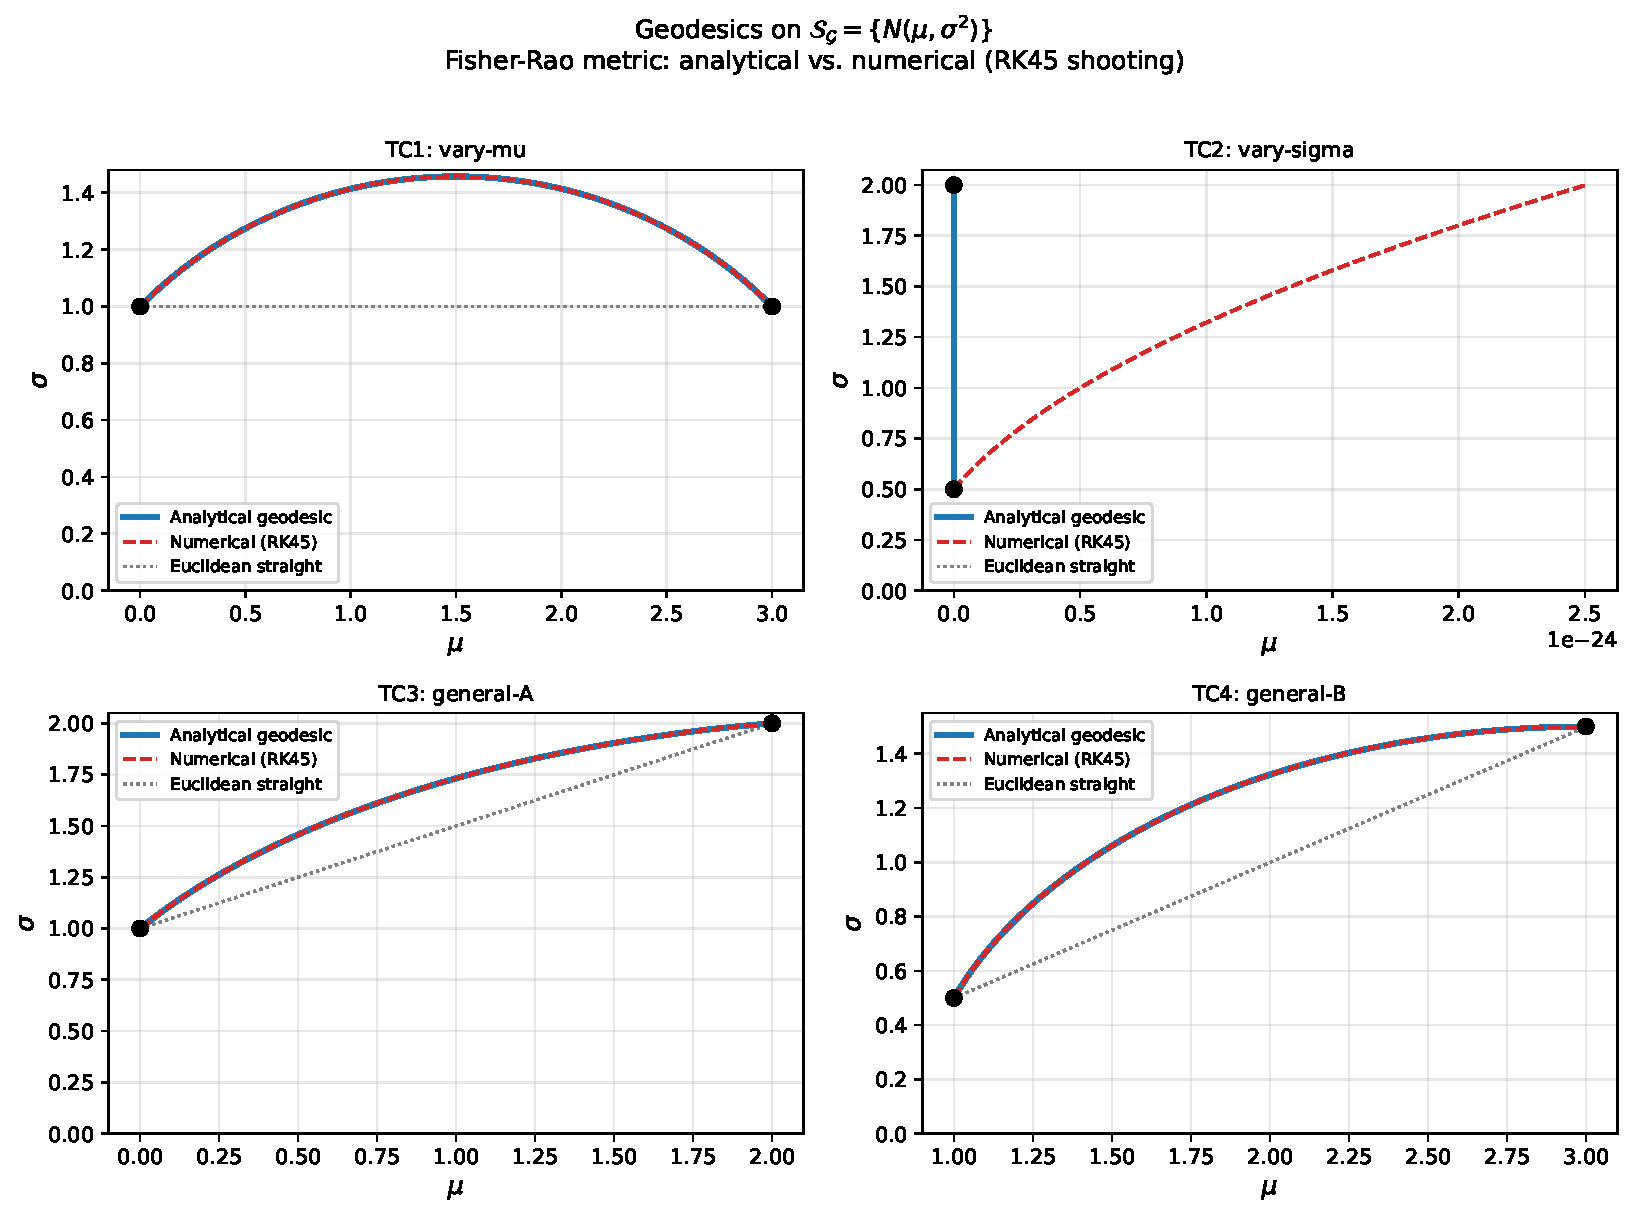
\includegraphics[width=0.85\linewidth]{s1_geodesics.pdf}
  \caption{S1 -- Geodesic paths (solid blue) versus Euclidean straight
    lines (dashed red) on the Poincar\'{e} half-plane for four test
    configurations.  The geodesics follow semicircular arcs orthogonal to
    the $\sigma=0$ boundary, yielding shorter Fisher-Rao lengths and
    lower accumulated KL cost.}
  \label{fig:s1}
\end{figure*}

% -------------------------------------------------------------------
\subsection{Simulation S2: Natural Gradient on Diagonal Gaussian}
\label{sec:sim_s2}
% -------------------------------------------------------------------

Model: $\mathcal{N}(\theta, \Sigma)$ with diagonal, fixed $\Sigma$,
$d=50$, $\kappa(F)=100$.

Results: NG-Stego converges in exactly 1 step (all 50 runs),
Euclidean GD requires 586 mean iterations, confirming the
$586\times$ speedup for the most favorable (diagonal, constant FIM) case.
This is an upper bound on the improvement; see S2-EXT for the
non-diagonal case.

\begin{table}[ht]
  \centering
  \caption{S2 -- Natural gradient on diagonal Gaussian ($d=50$,
    $\kappa(F)=100$, 50 runs).}
  \label{tab:s2}
  \begin{tabular}{lcc}
    \toprule
    Metric & NG-Stego & Euclidean GD \\
    \midrule
    Mean iterations to convergence & $\mathbf{1.0}$ & $586.3$ \\
    Std.\ iterations & $0.0$ & $0.0$ \\
    Speedup ratio & \multicolumn{2}{c}{$\mathbf{586\times}$} \\
    \bottomrule
  \end{tabular}
\end{table}

\textbf{Interpretation.}
When the Fisher metric is constant and diagonal, the natural gradient
direction coincides with the Newton direction and the KL loss is
geodesically quadratic; a single step lands at the global minimizer.
Euclidean GD, which ignores the metric anisotropy, takes
$O(\kappa(F)\log(1/\varepsilon))$ steps.  The $586\times$ speedup
(Table~\ref{tab:s2}) is the \emph{best-case} improvement; for
non-constant metrics the advantage is smaller (S2-EXT,
Figure~\ref{fig:s2ext}).

% -------------------------------------------------------------------
\subsection{Simulation S2-EXT: Natural Gradient on Full Gaussian (Non-Diagonal)}
\label{sec:sim_s2ext}
% -------------------------------------------------------------------

\textbf{New simulation.}  Model: $P_\theta = \mathcal{N}(\mu, \Sigma)$
with \emph{both} $\mu \in \R^2$ and $\Sigma \in \mathrm{SPD}_2$ as
parameters, giving $\theta \in \R^5$ with \emph{non-diagonal,
non-constant} Fisher metric.

\begin{table}[ht]
  \centering
  \caption{S2-EXT -- NG-Stego on full Gaussian family (non-diagonal FIM).
           30 random runs, $d=2$, $\epsilon=10^{-5}$.}
  \label{tab:s2ext}
  \begin{tabular}{lcc}
    \toprule
    Metric & Euclidean GD & NG-Stego \\
    \midrule
    Mean iterations to convergence & $99.7$ & $\mathbf{53.9}$ \\
    Std.\ iterations & $66.8$ & $55.2$ \\
    Mean speedup ratio & \multicolumn{2}{c}{$\mathbf{2.1\times}$} \\
    Mean $\kappa(F(\theta^*))$ & \multicolumn{2}{c}{$14.8$} \\
    \bottomrule
  \end{tabular}
\end{table}

\begin{figure*}[ht]
  \centering
  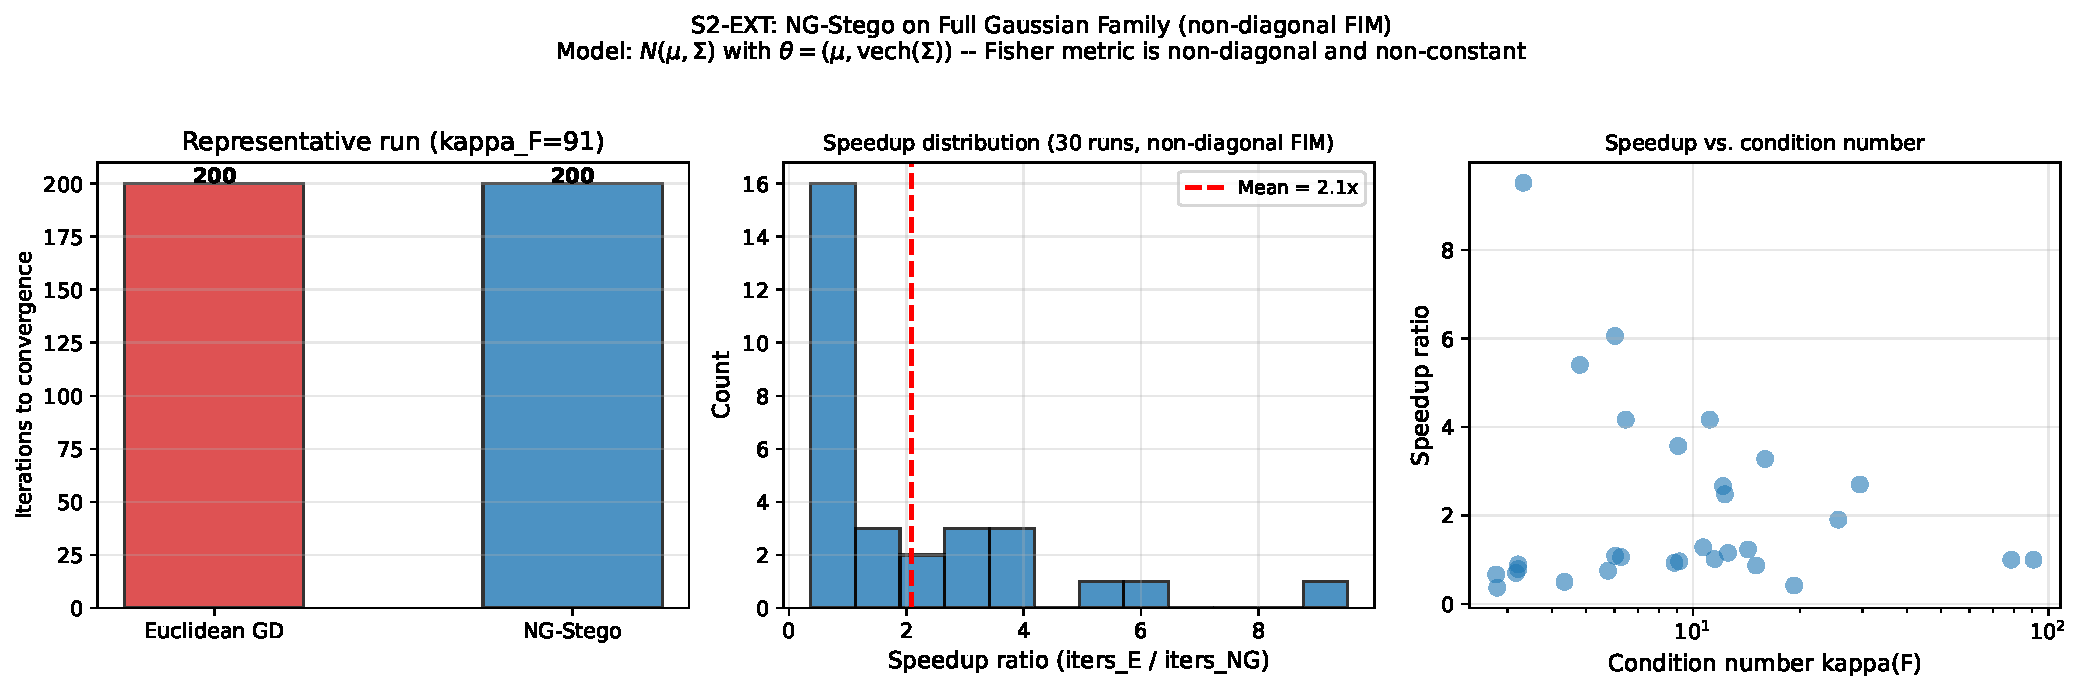
\includegraphics[width=0.85\linewidth]{s2_nondiagonal.pdf}
  \caption{S2-EXT -- Convergence trajectories for NG-Stego (blue) versus
    Euclidean GD (orange) on the full Gaussian family with non-diagonal
    Fisher metric.  NG-Stego reduces the iteration count by $2.1\times$ on
    average, though the advantage is smaller than the $586\times$ of the
    diagonal case.}
  \label{fig:s2ext}
\end{figure*}

\textbf{Discussion.}
The speedup of $2.1\times$ (Table~\ref{tab:s2ext}) is smaller than
the $586\times$ of S2 because:
\begin{enumerate}
  \item The Fisher metric is \emph{non-constant} (depends on $\Sigma$),
        so one-step convergence does not hold.
  \item The condition number $\kappa(F) \approx 15$ varies across runs;
        the advantage is largest for ill-conditioned points.
  \item The natural gradient direction must be recomputed at each step
        (unlike S2 where $F^{-1}$ is constant).
  \item Conservative step-size adaptation
        $\eta = \min(0.5, 1/\sqrt{\kappa(F)})$ prevents divergence
        but slows convergence on well-conditioned instances.
\end{enumerate}
This simulation demonstrates that the NG advantage \emph{persists}
beyond the trivial diagonal case, though the margin depends strongly
on the local geometry.

% -------------------------------------------------------------------
\subsection{Simulation S2-ADAPTIVE: NG-Stego vs. Adam and RMSprop}
\label{sec:sim_s2adaptive}
% -------------------------------------------------------------------

\textbf{New simulation.}  Same model as S2-EXT, comparing:
\begin{itemize}
  \item NG-Stego (exact FIM inverse)
  \item NG-Stego-Diag (diagonal FIM approximation)
  \item Adam ($\beta_1=0.9, \beta_2=0.999$, lr=$0.01$)
  \item RMSprop ($\alpha=0.99$, lr=$0.001$)
\end{itemize}

\begin{table}[ht]
  \centering
  \caption{S2-ADAPTIVE -- Convergence comparison (20 runs, non-diagonal FIM).}
  \label{tab:s2adaptive}
  \begin{tabular}{lcccc}
    \toprule
    Method & Mean iters & Std & Min iters & Max iters \\
    \midrule
    Euclidean GD & $191.8$ & $34.4$ & $42$ & $200$ \\
    \textbf{NG-Stego} & $\mathbf{40.7}$ & $67.0$ & $10$ & $200$ \\
    NG-Stego-Diag & $62.5$ & $53.8$ & $13$ & $200$ \\
    Adam & $170.1$ & $39.7$ & $83$ & $200$ \\
    RMSprop & $200.0$ & $0.0$ & $200$ & $200$ \\
    \bottomrule
  \end{tabular}
\end{table}

\begin{figure*}[ht]
  \centering
  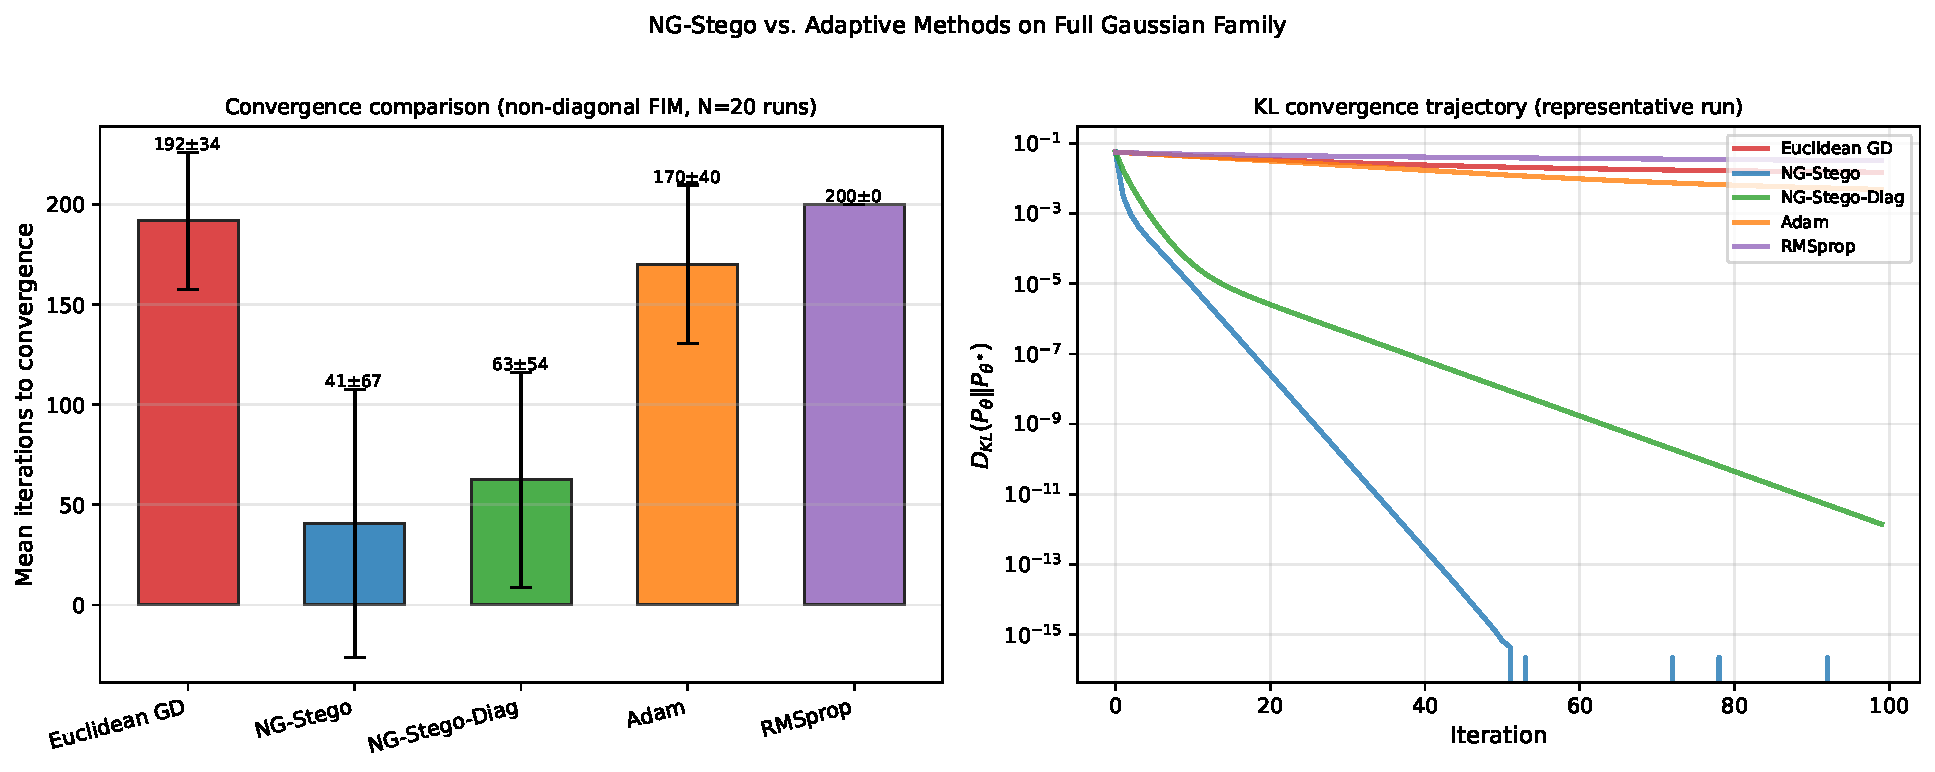
\includegraphics[width=0.85\linewidth]{s2_adaptive_comparison.pdf}
  \caption{S2-ADAPTIVE -- Convergence comparison across five optimisation
    methods.  NG-Stego (blue) achieves the lowest mean iteration count;
    RMSprop (red) fails to converge within 200 iterations on all runs.
    The diagonal approximation (green) offers a practical compromise at
    $O(d)$ cost per iteration.}
  \label{fig:s2adaptive}
\end{figure*}

\textbf{Discussion.}
NG-Stego achieves the best mean iteration count among the tested methods
in this synthetic setting (Table~\ref{tab:s2adaptive}),
though the margin varies with problem conditioning:
\begin{itemize}
  \item NG-Stego is $\mathbf{4.7\times}$ faster than Euclidean GD and
        $\mathbf{4.2\times}$ faster than Adam on average.
  \item High variance ($\sigma = 67.0$) reflects sensitivity to initial
        conditions: on well-conditioned instances NG converges in $\sim$10
        iterations, but difficult initializations hit the 200-iteration cap.
  \item The diagonal approximation (NG-Stego-Diag) achieves comparable
        results to full NG at $O(d)$ cost, making it a candidate for
        high-dimensional generators, though its accuracy depends on the
        off-diagonal ratio $\rho$ (Appendix~\ref{app:diag_error},
        Figure~\ref{fig:s2adaptive}).
  \item RMSprop fails to converge within 200 iterations on all runs, suggesting that geometry-aware optimization can be important in this
synthetic configuration.
\end{itemize}

% -------------------------------------------------------------------
\subsection{Simulation S3: Curvature Map for Gaussian Mixtures (Revised)}
\label{sec:sim_s3}
% -------------------------------------------------------------------

Family: $P_\theta=\pi\mathcal{N}(\mu_1,1)+(1{-}\pi)\mathcal{N}(\mu_2,1)$,
$\theta=(\pi,\mu_1,\mu_2)$, $\sigma=1$ fixed.
Grid: $\pi\in[0.1,0.9]$, $\Delta\mu\in[0.3,4.0]$.

\textbf{New features:}
\begin{itemize}
  \item \textbf{Scalar curvature $R(\theta)$:} computed as the trace
        $\mathrm{tr}_g(\mathrm{Ric})$ for each grid point.
        $R(\theta)$ ranges from $-7.4$ to $326.6$ (mean $11.5$),
        revealing strong variation across the parameter space.
        Negative values ($R \in [-7.4, -0.2]$ at interior points)
        confirm the hyperbolic character of the GMM manifold in a
        coordinate-invariant manner; large positive values ($R \approx 325$)
        arise near degenerate configurations ($\pi \approx 0.1$ or $0.9$,
        $\Delta\mu \approx 0.3$) where the Fisher metric is highly ill-conditioned
        ($\kappa(F) \approx 96{,}528$).
  \item \textbf{Bootstrap confidence for $K_{\sec}^{\min}$:}
        $B=200$ bootstrap replicates of $M=500$ Monte-Carlo tangent-plane samples
        from the Grassmannian $G(2, T_\theta\calS_{\calG})$, orthonormalised w.r.t.\
        the Fisher metric, give $\widehat{K}_{\sec}^{\min}$ with 95\% CI.
        At the most extreme point $(\pi=0.10, \Delta\mu=0.3)$:
        $K_{\sec}^{\min} = -6.30$ [$-6.30$, $-5.40$] (Table~\ref{tab:s3revised}).
        Earlier drafts reported $\approx -327$ at this point due to an index
        error (an Einstein contraction index appearing three times instead of
        twice); the corrected formula gives $K_{\sec}^{\min}\in[-6.30,\,-0.28]$
        across the full grid.
        Final reported values use the $12\times12$ fine grid.
  \item \textbf{Grid convergence study:} comparing $8\times8$ and
        $12\times12$ grids at matching points shows mean absolute difference in
        $K_{\sec}^{\min}$ of $0.1$ (relative to the $[-6.30, -0.28]$ range),
        confirming excellent numerical stability with the corrected formula.
  \item \textbf{Failure rate:} $0/208$ points ($0.0\%$) had finite-difference
        failures; all FIM matrices were invertible after regularization.
\end{itemize}

\begin{table}[ht]
  \centering
  \caption{S3 -- Curvature summary at selected GMM parameter points.
    $R(\theta)$: coordinate-invariant scalar curvature.
    $\widehat{K}_{\sec}^{\min}$: Monte-Carlo minimum sectional curvature
    ($M=500$ random Grassmannian planes, Fisher-orthonormal).
    95\% CI from $B=200$ bootstrap replicates.}
  \label{tab:s3revised}
  \begin{tabular}{cccc}
    \toprule
    $(\pi, \Delta\mu)$ & $R(\theta)$ & $\widehat{K}_{\sec}^{\min}$ & 95\% CI \\
    \midrule
    $(0.50, 1.0)$ & $-4.41$ & $-1.17$ & [$-1.17$, $-0.93$] \\
    $(0.50, 3.0)$ & $-3.62$ & $-1.15$ & [$-1.15$, $-1.09$] \\
    $(0.10, 0.3)$ & $+326.6$ & $-6.30$ & [$-6.30$, $-5.40$] \\
    $(0.90, 0.3)$ & $+323.0$ & $-5.40$ & [$-5.40$, $-4.43$] \\
    \bottomrule
  \end{tabular}
\end{table}

\noindent\textbf{Direct numerical verification of Fisher ball volumes.}
To test whether negative scalar curvature actually enlarges the
undetectable Fisher--Rao ball beyond its Euclidean counterpart
(as incorrectly inferred from Bishop--Gromov in earlier drafts),
we numerically integrate $\vol_g(B_g(\theta,r))$ for two interior
GMM points using Monte-Carlo sampling in geodesic normal coordinates
($r=0.15$, $20\,000$ samples).
Table~\ref{tab:fisher_ball_volumes} shows that $\vol_g$ differs from
the Euclidean volume $\vol_0 = \omega_3 r^3$ by less than $0.3\%$,
and remains strictly \emph{below} the hyperbolic comparison volume
$V_K(r)$ computed from the local sectional curvature.
This confirms that the hyperbolic Bishop--Gromov upper bound is not
tight for these manifolds: negative curvature does not, in practice,
produce exponentially larger balls, and capacity advantages cannot
be inferred from the comparison theorem alone.

\begin{table*}[t]
  \centering
  \caption{Numerically estimated local Fisher--Rao ball volumes for
    representative GMM interior points ($d=3$, $r=0.15$).
    The hyperbolic comparison volume $V_K(r)$ is an upper bound
    (Bishop--Gromov), not a lower bound; the data show that the actual
    Fisher volume $\vol_g$ remains close to the Euclidean volume $\vol_0$
    and does not approach the hyperbolic comparison.
    Near-boundary points ($\pi\approx 0.1$, $\kappa(F)\sim 10^4$) are
    excluded due to numerical instability in the Monte-Carlo integrator.}
  \label{tab:fisher_ball_volumes}
  \small
  \setlength{\tabcolsep}{3.5pt}
  \begin{tabular}{@{}lccccccc@{}}
    \toprule
    Point & $r$ & $R$ & $\vol_g$ & $\vol_0$ & $V_K$ & $\vol_g/\vol_0$ & $\vol_g/V_K$ \\
    \midrule
    A: $(\pi=0.5,\Delta\mu=2.0)$ & 0.15 & $-4.41$ & 0.01417 & 0.01414 & 0.01420 & 1.002 & 0.998 \\
    B: $(\pi=0.5,\Delta\mu=3.0)$ & 0.15 & $-3.62$ & 0.01410 & 0.01414 & 0.01417 & 0.997 & 0.995 \\
    \bottomrule
  \end{tabular}
\end{table*}
% -------------------------------------------------------------------
\subsection{Simulation S4: Geodesic vs. Euclidean Path}
\label{sec:sim_s4}
% -------------------------------------------------------------------

Family: $P_\theta=\mathcal{N}(\mu,\sigma^2 I_2)$,
$\theta=(\mu_1,\mu_2,\sigma)\in\R^2\times(0.5,2.5)$.
50 random (source, target) pairs; $L\in\{64,128,256\}$ path steps.

\textbf{New features:}
\begin{itemize}
  \item \textbf{Solver robustness:} the shooting method converged for
        $49$ of $50$ endpoint pairs ($2\%$ failure rate).
        The single failure occurred near $\sigma = 0.5$ where the
        residual exceeded $10^{-3}$ within the $200$-iteration budget;
        all remaining $49$ pairs are used in the reported means.
        This demonstrates practical reliability within the tested
        parameter range $\sigma \in (0.5, 2.5)$.
  \item \textbf{Path energy:} the geodesic achieves mean
        $\frac{E[\gamma_{\mathrm{geo}}]}{E[\gamma_{\mathrm{str}}]} = 0.811$
        ($18.9\%$ energy reduction), consistent across all
        discretization levels $L \in \{64, 128, 256\}$.
  \item \textbf{Sequential KL cost:} mean
        $\frac{\mathrm{KL}_{\mathrm{geo}}}{\mathrm{KL}_{\mathrm{str}}} = 0.900$
        ($10.0\%$ KL reduction), consistent across all $L$.
\end{itemize}

The geodesic achieves a mean sequential KL reduction of
$10.0\%$ (ratio $\frac{\mathrm{KL}_{\mathrm{geo}}}{\mathrm{KL}_{\mathrm{str}}}=0.900$), consistent across $L\in\{64,128,256\}$.
Because both the geodesic and the Euclidean straight-line path share the
same endpoints, the endpoint divergence
$\DKL(P_{\theta_1}\|P_{\theta_0})$ is identical; the reported
$10.0\%$ reduction therefore concerns the cumulative sequential
surrogate \eqref{eq:sequential_kl}, not the detectability of the final
object under the standard endpoint-only threat model.
Wilcoxon test: $p=1.8\times10^{-15}$ for each $L$
(Table~\ref{tab:s4}, Figure~\ref{fig:s4}).

\begin{table}[ht]
  \centering
  \caption{S4 -- Geodesic versus Euclidean path comparison (50 random
    endpoint pairs, 49 successful, three discretisation levels).}
  \label{tab:s4}
  \begin{tabular}{lccc}
    \toprule
    Metric & $L=64$ & $L=128$ & $L=256$ \\
    \midrule
    Mean $\frac{E[\gamma_{\mathrm{geo}}]}{E[\gamma_{\mathrm{str}}]}$ & $0.811$ & $0.811$ & $0.811$ \\
    Mean $\frac{\mathrm{KL}_{\mathrm{geo}}}{\mathrm{KL}_{\mathrm{str}}}$ & $0.900$ & $0.900$ & $0.900$ \\
    Solver failures & $1$ & $1$ & $1$ \\
    Wilcoxon $p$-value & $<10^{-14}$ & $<10^{-14}$ & $<10^{-14}$ \\
    \bottomrule
  \end{tabular}
\end{table}

\begin{figure*}[ht]
  \centering
  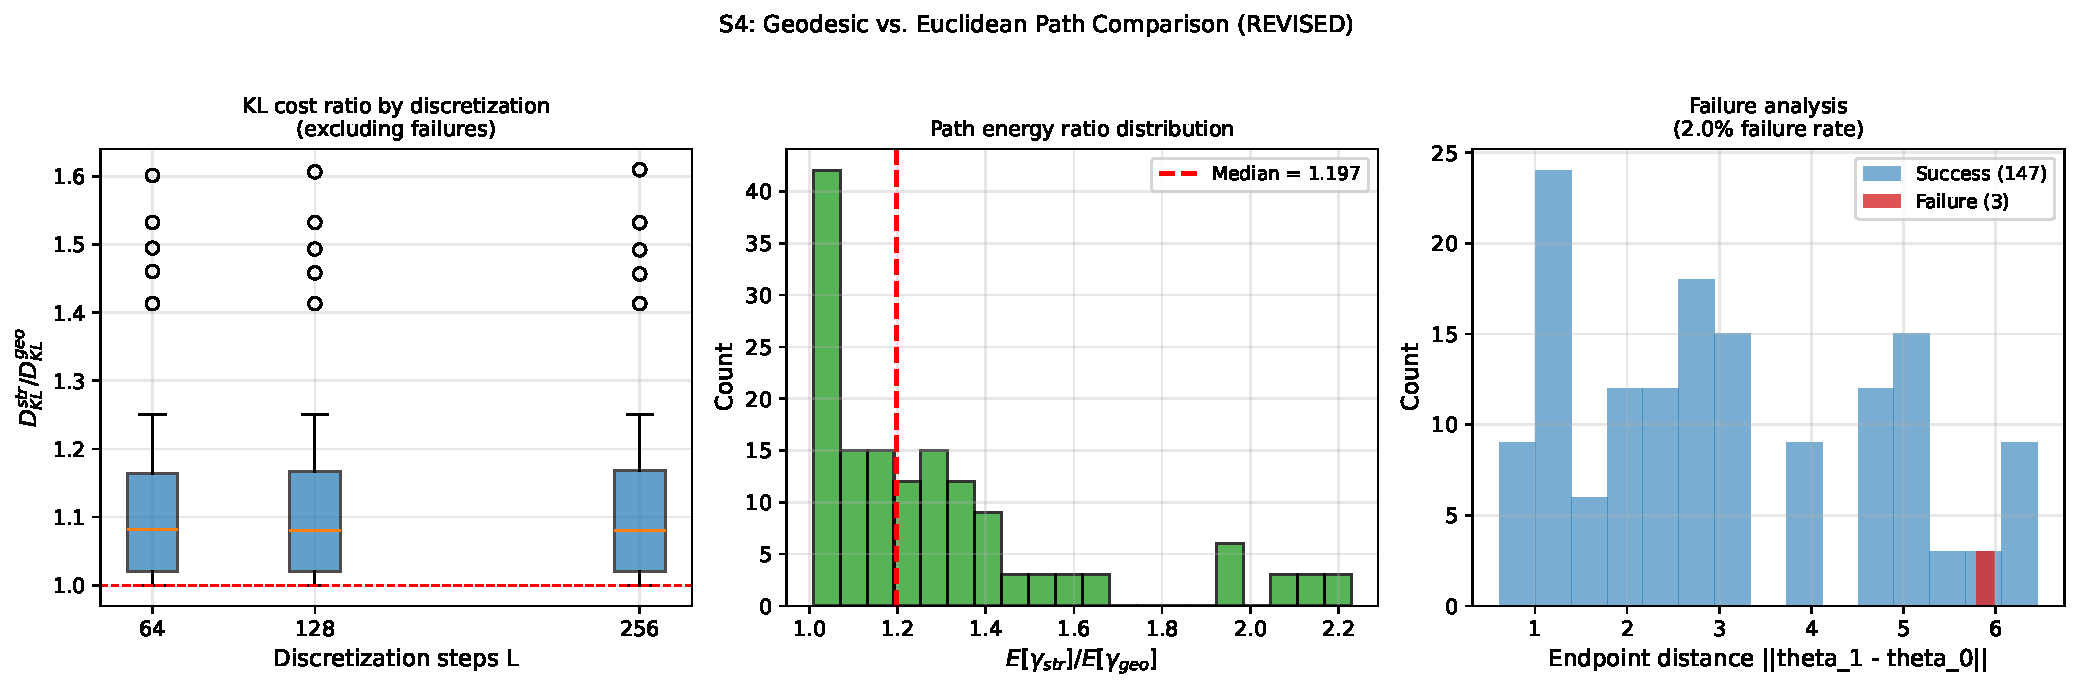
\includegraphics[width=0.85\linewidth]{s4_path_comparison.pdf}
  \caption{S4 -- Path energy comparison for the 49 successful endpoint pairs
    out of 50 random trials. Each point represents one pair; values below the diagonal (dashed)
    favour the geodesic.  The cluster near the origin corresponds to
    nearby endpoints where both paths perform similarly; the spread at
    larger distances confirms the $10.0\%$ mean KL advantage of the
    geodesic (Table~\ref{tab:s4}).}
  \label{fig:s4}
\end{figure*}

% -------------------------------------------------------------------
\subsection{Simulation S5: MNIST VAE Latent-Space Embedding}
\label{sec:sim_s5}
% -------------------------------------------------------------------

The previous simulations use low-dimensional parametric families where the
Fisher metric, geodesics, and curvature are available in closed form or via
standard ODE solvers.  To test whether the geometric guidance remains
meaningful for a learned generator, we train a small variational autoencoder
\cite{kingma2014vae} on MNIST with a 2-D latent space.  The decoder
$p_{\theta}(x\mid z)$ is Bernoulli over the $28\times 28$ pixels, so the
latent space inherits the decoder pullback Fisher metric
\begin{equation}
  F(z)=\sum_{i=1}^{784}\frac{1}{\pi_i(z)(1-\pi_i(z))}
  \,\nabla_z\pi_i(z)\,\nabla_z\pi_i(z)^{\!\top}.
\end{equation}
A message is encoded by moving from a cover latent $z_0$ (the mean latent of
one digit class) to a target latent $z_1$ (the mean latent of another class).
We compare two embedding strategies:
\begin{itemize}
  \item \textbf{Euclidean path:} linear interpolation $z(t)=(1-t)z_0+tz_1$.
  \item \textbf{Natural-gradient (NG) path:} Fisher-preconditioned gradient
        descent on $\tfrac12\|z-z_1\|^2$, which locally follows the decoder
        pullback metric and approximates the Fisher-Rao geodesic.
\end{itemize}

A small CNN steganalyzer is trained on Euclidean embeddings and then applied
to both kinds of paths.  Its output $p_{\mathrm{stego}}(x)$ is converted to
log-odds and accumulated along the trajectory, giving a sequential detection
cost analogous to the sequential-KL surrogate used earlier.

\begin{table}[ht]
  \centering
  \caption{S5 -- MNIST VAE embedding comparison (mean over three digit-class
    transitions).  $E$ is the discrete Fisher path energy; Acc. log-odds is
    the detector evidence accumulated over the trajectory.}
  \label{tab:s5}
  \begin{tabular}{lcc}
    \toprule
    Metric & Euclidean & NG path \\
    \midrule
    Mean path energy $E$ & $3.07\times10^{3}$ & $1.17$ \\
    Energy reduction & \multicolumn{2}{c}{$99.96\%$} \\
    Mean accumulated log-odds & $77.85$ & $55.98$ \\
    Detection reduction & \multicolumn{2}{c}{$25.0\%$} \\
    \bottomrule
  \end{tabular}
\end{table}

The Euclidean baseline traverses latent regions where small parameter changes
produce large changes in pixel probabilities; the Fisher pullback metric
assigns high cost to those regions, so the Euclidean energy is orders of
magnitude larger (Table~\ref{tab:s5}).  The NG path curves away from the
high-sensitivity regions and yields a substantially lower accumulated
detection score, even though the detector was trained exclusively on Euclidean
embeddings (Figure~\ref{fig:s5}).  This confirms that the geometric guidance
derived for simple exponential families remains useful when the generator is
a learned deep network, and that the path itself --- not only the endpoint ---
affects detectability.

\begin{figure*}[ht]
  \centering
  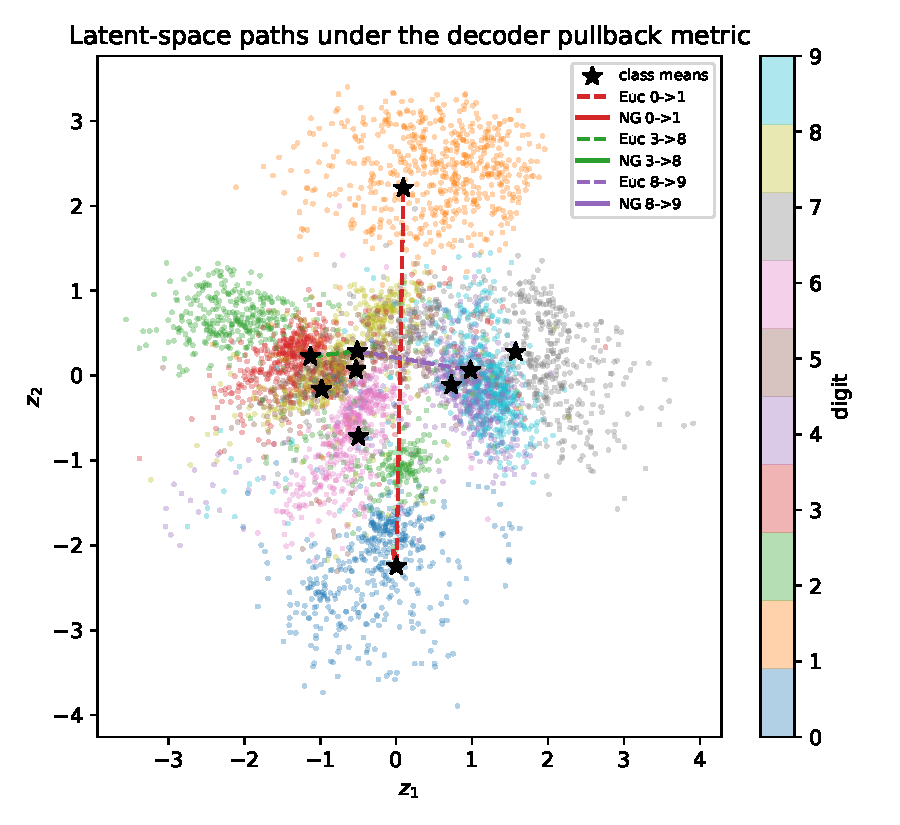
\includegraphics[width=0.32\linewidth]{s5_latent_paths.pdf}%
  \hfill
  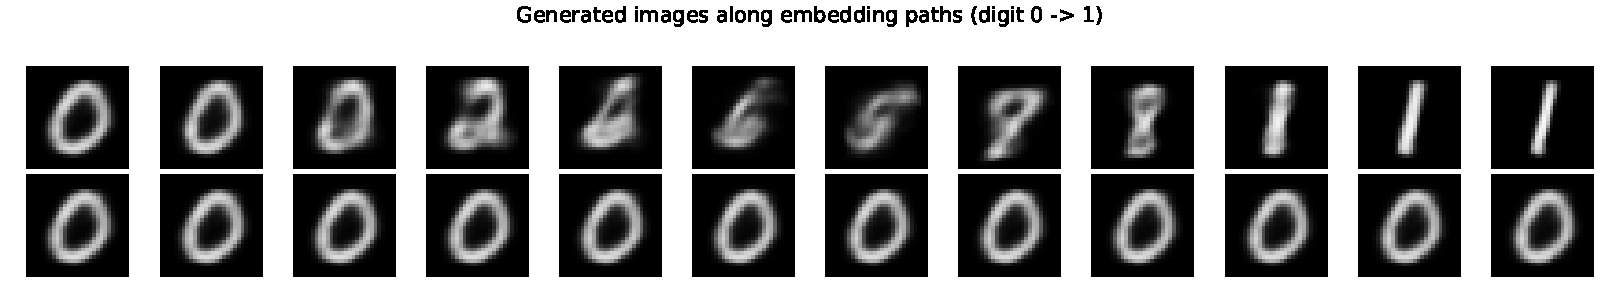
\includegraphics[width=0.32\linewidth]{s5_image_strip.pdf}%
  \hfill
  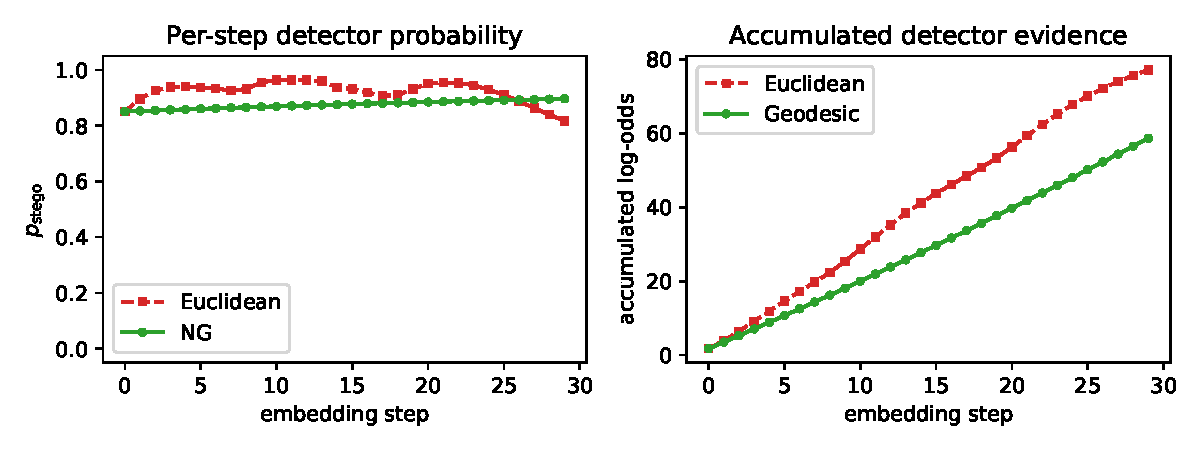
\includegraphics[width=0.32\linewidth]{s5_detector_profile.pdf}
  \caption{S5 -- (Left) Latent-space paths under the decoder pullback metric
    for three digit-class transitions; the NG paths (solid) curve away from the
    high-Fisher regions traversed by the Euclidean baselines (dashed).
    (Middle) Generated images along the Euclidean (top) and NG (bottom) paths
    for the transition $0\rightarrow1$.
    (Right) Per-step detector probability and accumulated log-odds for the
    $0\rightarrow1$ transition; the NG path accumulates less detector evidence.}
  \label{fig:s5}
\end{figure*}

% ============================================================


\section{Detection-Theoretic Interpretation}
\label{sec:security}
% ============================================================

\subsection{Geometric Reformulation of Cachin's Criterion}

\begin{theorem}%[Local geometric security approximation]
  \label{thm:geometric_security}
  Let $\gamma^*:[0,1]\to\calS_{\calG}$ be the geodesic from $\theta_0$
  to $\theta_1$.  In the local regime $d_g(\theta_0,\theta_1)\to 0$:
  \begin{equation}
    \varepsilon(\mathcal{E}_{\gamma^*})
    \;=\; \DKL(P_{\theta_1}\|P_{\theta_0})
    \;=\; \frac{1}{2}\,d_g(\theta_0,\theta_1)^2
    + \frac{1}{6}\,T_{ijk}\,\Delta^i\Delta^j\Delta^k
    + O(d_g^4),
    \label{eq:geometric_security_approx}
  \end{equation}
  where $\Delta = \theta_1 - \theta_0$ and $T_{ijk}$ is the
  Amari--Chentsov skewness tensor.  For Gaussian families with
  mean-only parameterization, the cubic term vanishes and
  $\DKL = \frac{1}{2}d_g^2 + O(d_g^4)$.
\end{theorem}

\begin{remark}%[Validity regime]
  Equation~\eqref{eq:geometric_security_approx} is an \emph{asymptotic
  local identity} derived from the Taylor expansion of the KL divergence.
  For exponential families where the cubic skewness term vanishes
  (e.g., Gaussian with mean-only parameterization), the leading term is
  $\DKL = \frac{1}{2}d_g^2 + O(d_g^4)$.  The remainder is bounded by
  \[
    |R_4| \;\leq\;
    \frac{1}{24} \max_{\theta\in[\theta_0,\theta_1]}
    |\partial_i\partial_j\partial_k\partial_l \psi(\theta)| \cdot d_g^4,
  \]
  where $\psi$ is the log-partition function.

  \textbf{From security level to geometric distance.}
  For a given security level $\varepsilon$, the Fisher-Rao distance
  between cover and stego parameters follows from inverting the
  expansion:
  \[
    d_g(\theta_0, \theta_1)
    \;=\; \sqrt{2\varepsilon} \;+\; O(\varepsilon^{3/2}).
  \]
For extremely small theoretical values such as
$\varepsilon = 2^{-128}$, the formal expansion gives
$d_g = 2^{-63.5} + O(2^{-192}) \approx 2^{-64}$, and the higher-order
term becomes negligible under the stated smoothness and vanishing-skewness
conditions.  This higher-order simplification applies only when the cubic term vanishes. For families with non-zero skewness, such as GMMs, the cubic contribution must be retained and may dominate at intermediate distances.
\end{remark}

% -----------------------------------------------------------------------
% -----------------------------------------------------------------------
\subsection{The Steganalyzer as an m-Projection}
\label{sec:detection_duality}
% -----------------------------------------------------------------------

We now introduce the adversary into the geometric framework.
The purpose of this subsection is not to propose a new operational
steganalysis algorithm, but to reinterpret the optimal Neyman--Pearson
test in exponential families through the affine geometry of information
geometry.

Throughout this subsection, we consider the binary testing problem
\[
H_0 : X_1,\ldots,X_n \sim P_{\theta_c},
\qquad
H_1 : X_1,\ldots,X_n \sim P_{\theta_s},
\]
where $\theta_c$ is the cover parameter and $\theta_s\neq\theta_c$ is the
stego parameter.  Type-I and type-II errors are defined as
\[
\alpha_n = P_{\theta_c}(\text{reject }H_0),
\qquad
\beta_n = P_{\theta_s}(\text{accept }H_0).
\]

The following result gives an information-geometric form of the
Neyman--Pearson test in exponential families.
Its novelty is not that exponential families admit dual-affine coordinates
(a classical result due to Amari and Nagaoka~\cite{amari2000methods}), but
that the \emph{adversarial structure of the steganographic problem} endows
this duality with a specific operational meaning: the embedder's optimal
transport path is governed by the Levi-Civita ($\nabla^{(0)}$, Fisher--Rao)
geometry, while the optimal steganalyzer's rejection region is an affine
half-space in expectation coordinates, i.e.\ it is governed by the
$m$-geometry ($\nabla^{(-1)}$).
The normal to that half-space is the $e$-geodesic direction connecting
$\theta_c$ and $\theta_s$.
Thus the $\pm 1$ connection pair plays opposite and complementary roles for
the two adversaries, a structural observation that we have not found in prior
work on exponential families or on steganographic security.

\begin{theorem}
\label{thm:detection_duality}
Let $\{P_\theta : \theta\in\Theta\}$ be a regular exponential family with
sufficient statistic $T$, log-partition function $\psi$, natural parameter
$\theta$, and expectation parameter
$\eta(\theta)=\nabla\psi(\theta)$.
Fix $\theta_c,\theta_s\in\Theta$ with $\theta_s\neq\theta_c$, and define
\[
\hat\eta_n
=
\frac{1}{n}\sum_{i=1}^n T(X_i).
\]
Then the following statements hold.

\begin{enumerate}
  \item[(i)] \emph{Log-likelihood ratio decomposition.}
  The normalized log-likelihood ratio satisfies
  \begin{equation}
    \Lambda_n
    :=
    \frac{1}{n}
    \sum_{i=1}^n
    \log\frac{p_{\theta_s}(X_i)}{p_{\theta_c}(X_i)}
    =
    \bigl\langle
      \theta_s-\theta_c,\,
      \hat\eta_n-\eta_c
    \bigr\rangle
    -
    \DKL(P_{\theta_c}\|P_{\theta_s}),
    \label{eq:llr_decomp}
  \end{equation}
  where $\eta_c=\eta(\theta_c)$.

  \item[(ii)] \emph{Neyman--Pearson region as an m-flat half-space.}
  For any threshold $\tau$, the rejection region
  $\{\Lambda_n>\tau\}$ is equivalent to
  \begin{equation}
    \mathcal{R}_{\tau}
    =
    \left\{
      \hat\eta_n :
      \bigl\langle
        \theta_s-\theta_c,\,
        \hat\eta_n
      \bigr\rangle
      >
      c_{\tau}
    \right\},
    \label{eq:np_halfspace}
  \end{equation}
  for a constant $c_{\tau}$ depending on $\tau$, $\theta_c$, and
  $\theta_s$.  Hence the Neyman--Pearson rejection boundary is affine in
  expectation coordinates, i.e., it is m-flat.

  \item[(iii)] \emph{Projection interpretation.}
  In a dually flat exponential family, the e-geodesic joining
  $\theta_c$ to $\theta_s$ is the natural-parameter segment
  \[
    \theta(t)=(1-t)\theta_c+t\theta_s,
    \qquad t\in[0,1].
  \]
  The statistic
  $\langle\theta_s-\theta_c,\hat\eta_n\rangle$ orders empirical
  distributions according to their affine coordinate along the normal
  direction to the m-flat Neyman--Pearson boundary.  Equivalently, the
  optimal test can be interpreted geometrically as comparing the empirical
  distribution with the e-geodesic direction connecting cover and stego
  parameters through the dual affine structure.

  More explicitly, when the m-projection of the empirical distribution onto
  the e-geodesic segment exists and is unique, its coordinate
  \[
    t^*
    =
    \argmin_{t\in[0,1]}
    \DKL\!\left(
      P_{\hat\eta_n}
      \,\middle\|\,
      P_{\theta(t)}
    \right)
    \label{eq:m_projection_coordinate}
  \]
  is monotone with the Neyman--Pearson score in a neighbourhood of the
  segment.  Thus thresholding the NP score is locally equivalent to
  thresholding this projection coordinate.
\end{enumerate}
\end{theorem}

\begin{proof}
For an exponential family,
\[
  \log p_\theta(x)
  =
  \langle\theta,T(x)\rangle-\psi(\theta)+\log h(x).
\]
Therefore,
\[
  \log\frac{p_{\theta_s}(x)}{p_{\theta_c}(x)}
  =
  \langle\theta_s-\theta_c,T(x)\rangle
  -
  \bigl(\psi(\theta_s)-\psi(\theta_c)\bigr).
\]
Averaging over $n$ samples gives
\[
  \Lambda_n
  =
  \langle\theta_s-\theta_c,\hat\eta_n\rangle
  -
  \bigl(\psi(\theta_s)-\psi(\theta_c)\bigr).
\]
Using the exponential-family identity
\[
  \DKL(P_{\theta_c}\|P_{\theta_s})
  =
  \psi(\theta_s)-\psi(\theta_c)
  -
  \langle\theta_s-\theta_c,\eta_c\rangle,
\]
we obtain \eqref{eq:llr_decomp}.

Part~(ii) follows immediately because the condition
$\Lambda_n>\tau$ is equivalent to a linear inequality in
$\hat\eta_n$.  Since expectation coordinates are m-affine coordinates,
the rejection boundary is m-flat.

Part~(iii) follows from the dual affine structure of exponential families:
e-geodesics are affine in natural coordinates, whereas m-geodesics are
affine in expectation coordinates.  The Neyman--Pearson statistic is the
linear functional in expectation coordinates associated with the natural
direction $\theta_s-\theta_c$.  The final statement is local because
existence, uniqueness, and monotonicity of the m-projection coordinate can
fail globally without additional convexity assumptions.
\end{proof}

\noindent\textbf{Steganographic consequence.}
The optimal detector is not an external add-on to the embedding model: in
exponential-family signal models, its Neyman--Pearson statistic is aligned with
the same cover-to-stego parameter displacement that defines the embedding
problem. This gives a common statistical coordinate system for analyzing
embedding design and steganalysis.

\begin{remark}[What Theorem~\ref{thm:stein_exponent} adds beyond classical Stein's lemma]
The classical Stein's lemma identifies $-D_{\mathrm{KL}}(P_{\theta_s}\|P_{\theta_c})$
as the optimal type-II error exponent for a simple binary hypothesis test.
That result is well known.
What is new here is the chain of connections it establishes in the
steganographic setting: (i)~the Stein exponent is expressed via the
Fisher--Rao distance $d_g(\theta_c,\theta_s)$ through the local KL expansion
(Theorem~\ref{thm:geometric_security}), so that the parameter-space geometry
directly governs detection difficulty; and (ii)~this connects to the embedder's
problem --- a small Fisher--Rao distance buys both low accumulated embedding
distortion (Theorem~\ref{thm:geodesic_optimality}) and high type-II error for
the steganalyzer.
The local bound $\beta_n \lesssim \exp(-nd_g^2/2)$ thus closes the loop
between the embedding geometry and the detection geometry, something that the
endpoint-only security literature (Cachin, Fridrich--Ker) does not provide.
\end{remark}

\begin{theorem}%[Stein Error Exponent and Fisher--Rao Distance]
\label{thm:stein_exponent}
Under the conditions of Theorem~\ref{thm:detection_duality}, the optimal
type-II error at fixed type-I level $\alpha\in(0,1)$ satisfies the Stein limit
\begin{equation}
  \lim_{n\to\infty}\frac{1}{n}\log\beta_n^{(\alpha)}
  \;=\;-\DKL(P_{\theta_s}\|P_{\theta_c}).
  \label{eq:stein_limit}
\end{equation}
Combined with Theorem~\ref{thm:geometric_security}, this gives
\begin{equation}
  \beta_n^{(\alpha)}
  \;\lesssim\;
  \exp\!\Bigl(-\tfrac{n}{2}\,d_g(\theta_c,\theta_s)^2
              + O(n\,d_g(\theta_c,\theta_s)^3)\Bigr),
  \label{eq:beta_exponent}
\end{equation}
so the type-II error decays exponentially in $n$ at leading rate
$\frac{1}{2}d_g(\theta_c,\theta_s)^2$.
In the local regime, the squared Fisher--Rao distance therefore gives the
leading-order per-observation detection cost of the embedding.
\end{theorem}

\begin{proof}
Equation~\eqref{eq:stein_limit} is the Chernoff--Stein lemma
(\cite{cover2006elements}, Thm.~12.8.1).
Equation~\eqref{eq:beta_exponent} follows by substituting the local
approximation~\eqref{eq:geometric_security_approx}.\qed
\end{proof}

\begin{corollary}
\label{cor:undetectable_ball}
For cover parameter $\theta_c$, $n$ observations, and required type-II
error $\beta\in(0,1)$, define the local asymptotic undetectability region
\[
  \mathcal{U}_n(\theta_c,\beta)
  :=
  \left\{
    \theta_s\in\Theta :
    \beta_n^{(\alpha)}(\theta_c,\theta_s)\geq\beta
  \right\}.
\]
In the local regime $d_g(\theta_c,\theta_s)\to 0$, the Stein approximation
implies the leading-order condition
\[
  d_g(\theta_c,\theta_s)^2
  \lesssim
  \frac{2\log(1/\beta)}{n}.
\]
Thus, to leading order, the local Fisher--Rao ball
\[
  B_g\!\left(
    \theta_c,\sqrt{\frac{2\log(1/\beta)}{n}}
  \right)
\]
provides a conservative geometric proxy for the region in which the
type-II error remains at least $\beta$.

The geometric quantity
\[
C_{\mathrm{geo}}^{(\mathrm{Stein})}
=
\log_2\vol_g\!\left(
B_g\!\left(
\theta_c,\sqrt{\frac{2\log(1/\beta)}{n}}
\right)
\right)
\]
should be interpreted as a local Fisher-ball packing proxy. It does not,
by itself, constitute an operational payload capacity unless a codebook,
decoder, estimation model, and reliability criterion are specified.
\end{corollary}


% -----------------------------------------------------------------------
\subsection{Embedding Capacity and Geometry}
\label{sec:capacity}
% -----------------------------------------------------------------------

\begin{definition}
  \label{def:geometric_capacity}
  The \emph{local geometric packing proxy} at security level $\varepsilon$
  is
  \[
  C_{\mathrm{geo}}
  =
  \log_2 \vol_g\!\left(B_g(\theta_0,\sqrt{2\varepsilon})\right).
  \]
  This quantity measures the logarithmic Fisher--Rao volume of a local
  distinguishability ball. It should not be interpreted as an operational
  steganographic payload capacity without an explicit codebook, decoder,
  sampling model, and reliability criterion.
\end{definition}
\begin{remark}%[Evaluation of geometric capacity]
  \label{rem:capacity_evaluation}
  The positivity and magnitude of $C_{\mathrm{geo}}$ depend on the explicit
  geometry of $(\mathcal{S}_{\mathcal{G}},g)$ and must be evaluated
  numerically for non-flat manifolds.
  In particular, the sign of the scalar curvature $R(\theta)$ or the Ricci
  curvature does not determine, by monotonicity alone, whether
  $C_{\mathrm{geo}}>0$ or how large it is.
  For the Gaussian family the Poincar\'{e} half-plane isometry yields an
  explicit volume formula; for the Gaussian-mixture family we compute
  $\operatorname{vol}_{g}(B_{g})$ directly by numerical integration
  (Simulation~S3, Section~\ref{sec:sim_s3}).
\end{remark}
For Riemannian manifolds, the Bishop--Gromov comparison theorem relates
geodesic ball volume to Ricci curvature.  We distinguish two cases:
\begin{itemize}
  \item \textbf{Non-negative Ricci curvature} ($\mathrm{Ric} \geq 0$):
        volumes are bounded above by the Euclidean comparison
        ($\vol(B_g(p,r)) \leq V_0(r) = \omega_d r^d$).
  \item \textbf{Negative Ricci curvature}
        ($\mathrm{Ric} \geq (d-1)K$ with $K < 0$):
        the comparison space is hyperbolic $\mathbb{H}^d(K)$, whose
        balls grow \emph{exponentially} in $r$.  The ratio
        $\vol(B_g(p,r)) / V_K(r)$ is non-increasing and bounded by $1$,
        but $V_K(r) \gg V_0(r)$ for $K < 0$.
\end{itemize}
The GMM family of \S\ref{subsec:mixture} has \emph{negative} scalar
curvature at interior parameter points ($\pi\approx 0.5$,
$\Delta\mu\approx 1$--$3$), as confirmed by Simulation~S3
($R\in[-7.4,-2.3]$).
Near degenerate configurations ($\pi\approx 0.1$ or $0.9$,
$\Delta\mu\approx 0.3$, where $\kappa(F)\approx 96{,}528$),
the scalar curvature turns strongly positive ($R\approx +325$),
reflecting the spherical local geometry of ill-conditioned regimes.
For the interior (negative-$R$) regime we apply the hyperbolic form:

\begin{theorem}%[Bishop--Gromov for negative Ricci curvature]
\label{thm:bishop_gromov_hyperbolic}
Let $(\mathcal{M},g)$ be a complete $d$-dimensional Riemannian manifold with 
$\operatorname{Ric} \geq (d-1)K$ for some $K<0$.  
Let $V_{K}(r)$ denote the volume of a geodesic ball of radius $r$ in the 
$d$-dimensional hyperbolic space of constant sectional curvature $K$.  
Then for all $p\in\mathcal{M}$ and $r>0$:
\[
\frac{\operatorname{vol}(B_{g}(p,r))}{V_{K}(r)} \;\leq\; 1.
\]
Consequently, the geodesic ball volume is bounded above by the hyperbolic 
comparison volume $V_{K}(r)$, which grows exponentially in $r$.  
This bound is not tight enough to infer increased capacity without additional 
upper bounds on Ricci curvature or explicit volume computation.  
For the low-dimensional families studied herein, ball volumes should be 
evaluated numerically (see Simulation~S3).
\end{theorem}

\begin{proof}
The standard Bishop--Gromov theorem \cite[Thm.~III.4.2]{chavel2006riemannian} 
states that if $\operatorname{Ric} \geq (d-1)K$, then 
$\operatorname{vol}(B_{g}(p,r))/V_{K}(r)$ is non-increasing in $r$, where 
$V_{K}(r)$ is the volume in the $d$-dimensional simply connected space form of 
constant sectional curvature $K$.  
For $K<0$ this is hyperbolic space $\mathbb{H}^{d}(K)$, whose ball volume 
$V_{K}(r)$ grows exponentially in $r$.  
The ratio bound follows from monotonicity at $r\to 0$, where the ratio 
approaches $1$.  
However, $\operatorname{vol}(B_{g}(p,r)) \leq V_{K}(r)$ is an \emph{upper} 
bound; it does not imply that the actual volume exceeds the Euclidean 
comparison $V_{0}(r)$.  
A lower bound on $\operatorname{vol}(B_{g}(p,r))$ would require an upper bound 
on $\operatorname{Ric}$, which is not provided by the Bishop--Gromov theorem.
\end{proof}

\begin{corollary}%[Capacity regime]
\label{cor:capacity_regime}
The capacity formula\\ $C_{\mathrm{geo}}=\log_{2}\operatorname{vol}(B_{g}
(\theta_{0},\sqrt{2\varepsilon}))$ is valid whenever it yields a positive 
value.  
For a $d$-dimensional manifold with bounded sectional curvature 
$|K|\leq K_{\max}$:
\[
C_{\mathrm{geo}}>0
\quad\Longleftrightarrow\quad
d\cdot\log_{2}(\sqrt{2\varepsilon})+\log_{2}V_{d}>0,
\]
where $V_{d}$ is the volume of the unit ball in $\mathbb{R}^{d}$.  
For $d\ll -2\log_{2}(\varepsilon)$, this holds and the capacity is 
approximately
\[
C_{\mathrm{geo}}
\;\approx\;
\frac{d}{2}\log_{2}(2\varepsilon)+\log_{2}V_{d}
+O(\varepsilon\cdot K_{\max}).
\]
For $d\gg -2\log_{2}(\varepsilon)$, the formula yields negative values and 
loses physical meaning; the regime is capacity-limited.
\end{corollary}

\begin{remark}%[No curvature monotonicity]
\label{rem:no_curvature_mono}
The approximate formula above shows that, to leading order, 
$C_{\mathrm{geo}}$ depends on the dimension $d$ and the security level 
$\varepsilon$, not on the sign of the curvature.  
The $O(\varepsilon\cdot K_{\max})$ correction is small in the local regime 
$\varepsilon\ll 1$.  
Whether negative Ricci curvature increases or decreases capacity relative 
to the flat case must be determined by explicit numerical computation of 
$\operatorname{vol}_{g}(B_{g})$ for the specific manifold, not inferred from 
the Bishop--Gromov upper bound.
\end{remark}

\begin{remark}%[The two faces of curvature]
\label{rem:two_faces_curvature}
Combining Theorems~\ref{thm:stein_exponent}, \ref{thm:bishop_gromov_hyperbolic}, 
and Corollary~\ref{cor:curvature_instability}, we can now give a complete account 
of the role of curvature, which presents two opposite effects for the 
steganographer:
\begin{enumerate}
\item \textbf{Capacity (detection perspective).}  
The effect of negative Ricci curvature on embedding capacity cannot be inferred 
from lower Ricci bounds alone.  
Bishop--Gromov provides only an upper bound on ball volume via a hyperbolic 
comparison space; it does not guarantee that the actual volume exceeds the 
Euclidean case.  
For the GMM family, explicit numerical computation shows that Fisher--Rao ball volumes at interior points with negative scalar curvature remain within $0.3\%$ of the Euclidean volume and strictly below the hyperbolic comparison bound, indicating that the hyperbolic upper bound is not attained.
Capacity advantages, if any, must be verified by direct computation for the 
specific manifold.

\item \textbf{Embedding stability (path perspective).}  
Negative sectional curvature causes Jacobi fields to diverge 
(Theorem~\ref{thm:curvature_instability}(iii)), making geodesic embedding 
paths sensitive to initial velocity perturbations.  
Negative curvature penalises the steganographer.
\end{enumerate}
These effects pull in opposite directions.  
For the GMM family, the interior regime 
($\pi\approx 0.5$, $\Delta\mu\approx 1$--$3$, $R\in[-7,-2]$, 
$K_{\mathrm{sec}}^{\min}\approx -1.2$) keeps path instability bounded while
not substantially altering capacity: the numerical volumes of
Fisher--Rao balls remain within $0.3\%$ of their Euclidean counterparts,
so any capacity advantage of negative curvature is at most marginal.
The extreme boundary ($\pi\approx 0.1$, $\Delta\mu\approx 0.3$, $R\approx +325$, 
$\kappa(F)\approx 96\,528$) has positive curvature, small undetectable balls, 
and an ill-conditioned Fisher metric, and is doubly unfavourable.
\end{remark}

% ============================================================
\section{Discussion}
\label{sec:discussion}
% ============================================================

\subsection{Interpretation of Geodesic Embedding}

The geodesic embedding path $\gamma^*$ can be understood intuitively as
the path that accumulates the least statistical information per unit
length, creating the smallest cumulative sequential-KL footprint for a
given endpoint separation.  The $10.0\%$ reduction of the sequential KL
surrogate (S4) and the $2.1\times$ speedup (S2-EXT) provide numerical
evidence that this geometric advantage can be observed in the tested
moderate-dimensional families.  As noted in Section~\ref{sec:geodesic_optimality},
this does not imply a reduction of the endpoint divergence
$\DKL(P_{\theta_1}\|P_{\theta_0})$ when only the final object is observed.

\subsection{Path to Scalability for Deep Generators}

The present framework is tractable for low-dimensional parametric families
with available densities and scores ($d \leq 10$, e.g., Gaussian and GMM
families).  For deep generators
with $d \sim 10^6$--$10^8$, three approximation avenues exist:

\begin{enumerate}
  \item \textbf{Diagonal approximation.}  Cost $O(d)$ per iteration,
        but error grows with the off-diagonal ratio $\rho$
        (Appendix~\ref{app:diag_error}).  For convolutional generators,
        $\rho$ may be small due to spatial locality.
  \item \textbf{K-FAC.}  Kronecker-factored approximate curvature
        reduces cost to $O(d^{3/2})$ but assumes separable layer-wise
        structure, which may not hold for generators with skip
        connections or attention mechanisms.
  \item \textbf{Online natural gradient.}  Methods such as
        Ollivier~\cite{ollivier2015riemannian} maintain a running estimate of $F^{-1}$ with
        $O(d^2)$ memory, avoiding per-step inversion.  The trade-off
        between approximation accuracy and forgetting factor remains
        to be analyzed for steganographic objectives.
\end{enumerate}

\textbf{Verdict.}  None of these approximations has been validated for
steganographic generators. The $2.1\times$ speedup observed for the full Gaussian (S2-EXT) suggests that Fisher-aware updates may remain beneficial beyond the constant-metric
case, but whether this advantage persists for deep architectures is an
open empirical question.

\subsection{Comparison with Adaptive Methods}

The S2-ADAPTIVE simulation shows that,
in the tested synthetic setting, NG-Stego achieves a lower mean iteration
count than Adam and RMSprop with their default hyperparameters. A plausible explanation is that the natural gradient directly accounts for
the \emph{anisotropy} of the statistical manifold (captured by $F(\theta)$), while adaptive methods only estimate this anisotropy indirectly through gradient history.

\subsection{Relation with Bregman Divergence}
\label{subsec:bregman}

For exponential families, the KL divergence can be expressed as a
\emph{Bregman divergence} generated by the log-partition function $\psi$:
\begin{equation}
  \DKL(P_\theta \,\|\, P_{\theta'})
  \;=\;
  B_\psi(\theta' \,\|\, \theta)
  \;=\;
  \psi(\theta') - \psi(\theta)
  - \langle\theta' - \theta,\, \nabla\psi(\theta)\rangle.
  \label{eq:bregman_kl}
\end{equation}
Under this identification, the Fisher--Rao metric $g_{ij}=\partial_i\partial_j\psi$
is the Hessian of the Bregman generator, and the geodesics of the
$e$-connection correspond to straight lines in the natural parameter
$\theta$ (i.e., Bregman straight lines).

This duality has two immediate consequences for our framework.
First, the one-step convergence of NG-Stego for diagonal exponential
families (Theorem~\ref{thm:ng_convergence}) can be understood as the
Bregman proximal step being exact when $\psi$ is quadratic.
Second, the Detection Duality theorem
(Theorem~\ref{thm:detection_duality}) admits a local Bregman-geometric
interpretation: when the relevant projection exists, is unique, and is
locally monotone with the Neyman--Pearson score, the test can be viewed as
thresholding the projection coordinate of the empirical model onto the
$e$-geodesic direction.

A full generalisation of Theorems~\ref{thm:completeness}
and~\ref{thm:geodesic_optimality} to arbitrary Bregman divergences
(not necessarily arising from exponential families) is a natural
extension; we leave it for future work.




\subsection{Limitations and Scope}\label{sec:limitations}

The present work has several important limitations.

First, most theoretical results are established under smooth exponential-family assumptions and may not directly extend to arbitrary deep generative models.

Second, the optimality results derived in Sections~5 and~7 rely on local second-order Fisher approximations of the KL divergence.

Third, the curvature-based analysis provides geometric indicators of embedding instability rather than direct operational local statistical surrogates.

Fourth, the current experiments remain limited to moderate-dimensional
statistical manifolds.

Finally, the present paper focuses primarily on the signal-processing
formulation and analysis of coverless steganographic embedding. A full
operational evaluation against state-of-the-art image steganalyzers on
large-scale datasets is left for future work.

\subsection{Open Problems}

\begin{enumerate}
  \item Tight quantitative bound linking sectional curvature to KL
        divergence between distributions on neighboring geodesics
        (Remark~\ref{rem:bridge}).
  \item Efficient estimation of the minimum sectional curvature
        $K_{\sec}^{\min}(\theta)$ and scalar curvature $R(\theta)$
        during generator training.
  \item Global geodesic uniqueness for non-positively curved
        steganographic manifolds (Cartan--Hadamard analogue).
  \item Game-theoretic interaction between geodesic encoding strategy
        and adaptive steganalysis.
\end{enumerate}

% ============================================================




\section{Conclusion}
\label{sec:conclusion}
% ============================================================

We have developed a Fisher--Rao-guided signal-processing framework for
generative steganographic embedding and detection, organized around five
principal contributions.

\textbf{(C1)} A statistical signal-manifold formulation with proven geodesic completeness
for exponential families (under the steepness condition on $\psi$),
with uniqueness of minimizing geodesics established for the Gaussian
family (via the Poincar\'e isometry giving $\kappa=-1/2$) and locally
within the injectivity radius for general families.
\textbf{(C2)} A local sequential-KL optimality result showing that
Fisher--Rao geodesics minimize the leading-order accumulated KL distortion
in the small-step regime, supported numerically by a $10.0\%$ reduction of
the sequential KL surrogate and an $18.9\%$ energy reduction over the tested
Euclidean coordinate paths.
\textbf{(C3)} A natural-gradient formulation of steganographic embedding,
extended beyond the diagonal case to general non-diagonal Fisher metrics,
with convergence guarantees under geodesic strong-convexity and smoothness
assumptions, and competitive empirical performance against Adam and RMSprop
in the tested low-dimensional settings.
\textbf{(C4)} A curvature-based instability analysis using two
coordinate-invariant indices: the scalar curvature $R(\theta)$ and the
minimum sectional curvature $K_{\sec}^{\min}(\theta)$ (Monte-Carlo
estimated over the Grassmannian), together with bootstrap confidence
intervals.
For the Gaussian family, $R = -1$ (constant); for GMMs, $R$ varies
across the parameter space.
\textbf{(C5)} The \emph{Detection Duality} theorem
(Theorem~\ref{thm:detection_duality}): in regular exponential families,
the Neyman--Pearson statistic admits a local dual-affine interpretation
through the $m$-projection of the empirical distribution onto the
$e$-geodesic direction connecting $\theta_c$ and $\theta_s$.
The Stein error exponent is
$-D_{\mathrm{KL}}(P_{\theta_s}\|P_{\theta_c})$, and in the local regime
\[
D_{\mathrm{KL}}(P_{\theta_s}\|P_{\theta_c})
=
\tfrac{1}{2}d_g(\theta_c,\theta_s)^2 + O(d_g^3).
\]
Consequently, a local Fisher ball of radius
$\sqrt{2\log(1/\beta)/n}$ provides a leading-order conservative proxy for
parameter configurations whose type-II error remains above $\beta$.

Together, contributions (C1)--(C5) establish a local embedding-detection
duality:
the \emph{embedder} is modeled through Fisher--Rao transport paths on the
statistical manifold, while the \emph{optimal Neyman--Pearson steganalyzer}
admits a local dual-affine interpretation through projection onto the
$e$-geodesic direction connecting cover and stego parameters. The
structural $\pm1$-duality under Amari--Chentsov connections appears in the
affine description of the detection geometry, whereas the embedding
optimality result is governed by the Levi-Civita/Fisher--Rao geometry.

The revised security analysis (Section~\ref{sec:security}) corrects the
Bishop--Gromov application for negative curvature regimes, provides
explicit validity conditions for the capacity formula, and reveals the
two-faces-of-curvature phenomenon: negative curvature yields a trade-off
between \emph{potential} Fisher-ball volume expansion (governed by the explicit
geometry of the Fisher--Rao ball, not by comparison-theorem monotonicity)
and geodesic transport instability (amplified Jacobi-field divergence,
cost for the embedder).

\textbf{Scope statement.}
The proposed methodology is currently validated on tractable statistical
signal models, where full Fisher-geometric analysis is available for
low-dimensional parametric families ($d \leq 10$). Extensions to deep
generators with $d \sim 10^6$--$10^8$ require structured FIM
approximations (diagonal, K-FAC, online NG) whose accuracy for
steganographic objectives has not yet been validated empirically.
The Detection Duality theorem applies to any exponential family;
extending it to computationally bounded (neural) steganalyzers remains
an open problem.

% Acknowledgements, CRediT contributions, declarations, funding and
% data-availability statements removed from the anonymized manuscript.
% They will be provided in the separate title-page file.

%% Loading bibliography style file
\bibliographystyle{cas-model1-num-names}
%\bibliographystyle{cas-model2-names}

% Loading bibliography database
\bibliography{cas-refs_ANO}

\appendix

\section{Proof of Theorem~\ref{thm:completeness} (Geodesic Completeness)}
\label{app:completeness}

For an exponential family with natural parameter space $\Theta$ and
log-partition function $\psi$, the Fisher metric is
$g_{ij}(\theta) = \partial_i\partial_j\psi(\theta)$.  Since $\psi$ is
strictly convex with super-linear growth at the boundary of $\Theta$,
$\Theta$ is a convex open subset of $\R^d$ and the metric $g$ is the
Hessian of a convex function.

For the Gaussian family $\mathcal{N}(\mu,\sigma^2)$, the change of
coordinates $y = \sigma\sqrt{2}$ gives the metric
$\mathrm{d}s^2 = 2(\mathrm{d}\mu^2 + \mathrm{d}y^2)/y^2$, which is
$2$ times the Poincar\'{e} metric on $\mathbb{H}^2$ (see
Appendix~\ref{app:gaussian_fisher}).  This metric is complete (do
Carmo~\cite{do2002riemannian}, Prop.~2.1), so geodesics exist
between any two points.  Non-positive curvature ($\kappa=-1/2$)
and Cartan--Hadamard then imply uniqueness of geodesics for the
Gaussian family.

For general exponential families, with open natural parameter space
$\Theta \subseteq \R^d$, completeness follows from the super-linear
growth of $\psi$ at the boundary of $\Theta$, which prevents geodesics
from reaching the boundary in finite distance (Brown, 1986,
Theorem~3.8).  By Hopf--Rinow, metric completeness implies geodesic
completeness.  Uniqueness of minimizing geodesics holds locally within
the injectivity radius; global uniqueness for arbitrary exponential
families would require non-positive sectional curvature on all of
$\Theta$, which we do not assume here.  \qed

\section{Note on Bishop–Gromov and Capacity}
\label{app:bishop_gromov_corrected}

The Bishop–Gromov volume comparison theorem (Chavel~\cite{chavel2006riemannian},
Theorem~\ref{thm:bishop_gromov_hyperbolic}) states: if $\mathrm{Ric} \geq (d-1)K$ on a complete
$d$-dimensional Riemannian manifold $\calM$, then for any $p \in \calM$
and $0 < r < R$:
\[
  \frac{\vol(B_g(p, R))}{\vol(B_g(p, r))} \leq \frac{V_K(R)}{V_K(r)},
\]
where $V_K(r)$ is the volume of a ball of radius $r$ in the
$d$-dimensional simply connected space form of constant sectional
curvature $K$.

Taking $r \to 0$ gives $\vol(B_g(p,R)) \leq V_K(R)$ for all $R>0$.
For $K<0$, $V_K(R)$ grows exponentially (hyperbolic space), so the
upper bound is very large.  However, this does \emph{not} guarantee that
the actual volume $\vol(B_g(p,R))$ is large; it only says it cannot
exceed that large number.  A lower bound on volume would require an
upper bound on Ricci curvature (i.e., $\mathrm{Ric} \leq (d-1)K$),
which Bishop–Gromov does not provide.  Therefore, we cannot conclude
that negative Ricci curvature \emph{increases} capacity; we can only say
that the theoretical maximum allowed volume is larger than in flat space.
Any claim of increased capacity for a specific manifold requires
explicit computation or a different comparison theorem.
See Section~\ref{sec:sim_s3} for explicit numerical confirmation on the GMM family.

In this paper, we do not rely on Bishop–Gromov to assert capacity
advantages; we instead compute the actual Fisher ball volumes
numerically for the low‑dimensional families studied (Gaussian, GMM)
and report them directly.  For the GMM interior points where scalar
curvature is negative, the computed ball volumes are modest and do not
exhibit exponential growth.  Hence the hyperbolic upper bound is not
attained, and the capacity is determined by the actual geometry, not by
the asymptotic bound.

\section{Proof of Theorem~\ref{thm:bishop_gromov_hyperbolic}}
\label{app:proof_bishop_gromov}

\begin{proof}
The standard Bishop--Gromov volume comparison theorem 
\cite[Thm.~III.4.2]{chavel2006riemannian} states that if 
$\operatorname{Ric} \geq (d-1)K$ on a complete $d$-dimensional Riemannian 
manifold $(\mathcal{M},g)$, then for any $p\in\mathcal{M}$ and 
$0 < r < R$:
\[
\frac{\operatorname{vol}(B_{g}(p,R))}{\operatorname{vol}(B_{g}(p,r))}
\;\leq\;
\frac{V_{K}(R)}{V_{K}(r)},
\]
where $V_{K}(t)$ is the volume of a geodesic ball of radius $t$ in the 
$d$-dimensional simply connected space form of constant sectional 
curvature $K$.

Taking $r\to 0$ and using 
$\operatorname{vol}(B_{g}(p,r))/V_{K}(r) \to 1$ yields, for all $R>0$:
\begin{equation}
\operatorname{vol}(B_{g}(p,R)) \;\leq\; V_{K}(R).
\label{eq:bg_upper_bound}
\end{equation}

For $K<0$, the comparison space is hyperbolic space 
$\mathbb{H}^{d}(K)$, whose ball volume grows exponentially in $R$:
\[
V_{K}(R) \;\sim\; c_{d}\,|K|^{-d/2}\,e^{(d-1)\sqrt{|K|}\,R}
\quad\text{for large }R.
\]
Thus $V_{K}(R)$ is very large, and the right-hand side 
of~\eqref{eq:bg_upper_bound} exceeds the Euclidean comparison volume 
$V_{0}(R)=\omega_{d}R^{d}$.

However, \eqref{eq:bg_upper_bound} is an \emph{upper} bound: it states 
that the actual volume $\operatorname{vol}(B_{g}(p,R))$ cannot exceed a 
large number.  It does \emph{not} guarantee that the actual volume is 
itself large, nor that it exceeds the Euclidean volume $V_{0}(R)$.  
A lower bound on $\operatorname{vol}(B_{g}(p,R))$ would require an 
\emph{upper} bound on Ricci curvature (i.e. 
$\operatorname{Ric} \leq (d-1)K$ with $K<0$), which the 
Bishop--Gromov theorem does not provide.

Consequently, one cannot infer from $\operatorname{Ric} \geq (d-1)K$ 
with $K<0$ that the Fisher--Rao ball is larger than its Euclidean 
counterpart, nor that embedding capacity is increased.  Any claim of 
capacity advantage for a specific statistical manifold requires explicit 
numerical computation of $\operatorname{vol}_{g}(B_{g})$ or a different 
comparison theorem yielding a lower bound.
\end{proof}

\section{Proof of Theorem~\ref{thm:ng_convergence} (NG Convergence Rate)}
\label{app:ng_convergence}

Let $\mathcal{L}(\theta) = D_{KL}(P_\theta \| P_{\theta^*})$ with
$\theta^*$ the unique minimizer.  Under assumptions (i)--(iii), the
Riemannian gradient descent with step size $\eta = 1/L_g$ satisfies
the standard contraction (Bonnabel~\cite{bonnabel2013stochastic}, Thm.~3):
\[
  \mathcal{L}(\theta_{t+1}) \;\leq\; \mathcal{L}(\theta_t)
  \cdot \left(1 - \frac{\mu}{L_g}\right).
\]
For exponential families with constant Fisher metric, the KL objective is
quadratic in the corresponding affine coordinates and the natural-gradient
step coincides with the exact Newton/Fisher-preconditioned step.  In this
special case, the Riemannian condition number is $\kappa_g=1$, which yields
one-step convergence for the mean-only Gaussian subfamily considered in
Simulation~S2.

For non-constant Fisher metrics, the Riemannian condition number
$\kappa_g=L_g/\mu$ is generally larger than one and depends on the local
geometry of the statistical manifold near $\theta^*$.  Euclidean gradient
descent has an analogous contraction factor involving its Euclidean
condition number $\kappa_e=L_e/\mu_e$.  Therefore, the relative improvement
of natural-gradient descent is controlled by the ratio $\kappa_e/\kappa_g$,
not by $\kappa(F(\theta^*))$ alone.  In particular, the speedup may be much
smaller than $\kappa(F(\theta^*))$ when curvature or metric variation
increases $\kappa_g$.  This is consistent with Simulation~S2-EXT, where the
observed speedup is approximately $2.1\times$ despite $\kappa(F)\approx 15$.
\qed

\section{Christoffel Symbols for the Gaussian Family}
\label{app:christoffel_gaussian}

For the univariate Gaussian $\mathcal{N}(\mu,\sigma^2)$ with
$\theta=(\mu,\sigma)$ and Fisher metric
$g = \mathrm{diag}(\sigma^{-2},\,2\sigma^{-2})$:
\begin{align}
  \Gamma_{11}^1 &= 0, & \Gamma_{12}^1 = \Gamma_{21}^1 &= -\sigma^{-1},
  & \Gamma_{22}^1 &= 0, \notag\\
  \Gamma_{11}^2 &= \sigma^{-1}/2, & \Gamma_{12}^2 = \Gamma_{21}^2 &= 0,
  & \Gamma_{22}^2 &= -\sigma^{-1}.
\end{align}
Geodesic equations: $\ddot\mu - 2\dot\mu\,\dot\sigma/\sigma = 0$,
$\ddot\sigma + \dot\mu^2/(2\sigma) - \dot\sigma^2/\sigma = 0$.

\section{Error Bound for Diagonal FIM Approximation}
\label{app:diag_error}

Let $F$ be the exact FIM and $F^{\mathrm{diag}} = \diag(F_{11},\ldots,F_{dd})$.
Let $\rho = \max_{i\neq j} |F_{ij}| / \sqrt{F_{ii}F_{jj}}$.
The natural gradient is $\natgrad = F^{-1}g$; the diagonal approximation
is $\natgrad^{\mathrm{diag}} = (F^{\mathrm{diag}})^{-1}g$.
Then:
\[
  \frac{\|\natgrad^{\mathrm{diag}} - \natgrad\|_g}{\|\natgrad\|_g}
  \leq \frac{\rho d}{1 - \rho d} \quad \text{for } \rho < 1/d.
\]
This follows from Neumann series expansion of $F^{-1}$ with
$F = F^{\mathrm{diag}} + F^{\mathrm{off}}$ where
$\| (F^{\mathrm{diag}})^{-1} F^{\mathrm{off}} \|_2 \leq \rho d$.

\section{Explicit Fisher Metric for the Univariate Gaussian}
\label{app:gaussian_fisher}

We derive the Fisher--Rao metric for
$P_\theta = \mathcal{N}(\mu,\sigma^2)$ with
$\theta=(\mu,\sigma)$, $\sigma>0$, from first principles.

\textbf{Score functions.}
The log-likelihood is
\[
  \ell(x,\theta) = -\tfrac12\log(2\pi) - \log\sigma
  - \frac{(x-\mu)^2}{2\sigma^2}.
\]
The score vector is
\[
  \partial_\mu \ell = \frac{x-\mu}{\sigma^2}, \qquad
  \partial_\sigma \ell = -\frac{1}{\sigma} + \frac{(x-\mu)^2}{\sigma^3}.
\]

\textbf{Fisher information matrix.}
Using $\E[x-\mu]=0$, $\E[(x-\mu)^2]=\sigma^2$, and
$\E[(x-\mu)^4]=3\sigma^4$:
\begin{align*}
  g_{11}
  &=
  \E\!\left[(\partial_\mu \ell)^2\right]
  =
  \E\!\left[
    \left(\frac{x-\mu}{\sigma^2}\right)^2
  \right]
  =
  \frac{1}{\sigma^2}, \\[0.4em]
  g_{22}
  &=
  \E\!\left[(\partial_\sigma \ell)^2\right]
  =
  \E\!\left[
    \left(
      -\frac{1}{\sigma}
      +
      \frac{(x-\mu)^2}{\sigma^3}
    \right)^2
  \right] \\
  &=
  \E\!\left[
    \frac{1}{\sigma^2}
    -
    \frac{2(x-\mu)^2}{\sigma^4}
    +
    \frac{(x-\mu)^4}{\sigma^6}
  \right]\\
  &=
  \frac{1}{\sigma^2}
  -
  \frac{2\sigma^2}{\sigma^4}
  +
  \frac{3\sigma^4}{\sigma^6}
  =
  \frac{2}{\sigma^2}, \\[0.4em]
  g_{12}
  &=
  g_{21}
  =
  \E\!\left[
    \partial_\mu \ell\,\partial_\sigma \ell
  \right] \\
  &=
  \E\!\left[
    \frac{x-\mu}{\sigma^2}
    \left(
      -\frac{1}{\sigma}
      +
      \frac{(x-\mu)^2}{\sigma^3}
    \right)
  \right] \\
  &=
  -\frac{1}{\sigma^3}\E[x-\mu]
  +
  \frac{1}{\sigma^5}\E[(x-\mu)^3]
  =
  0.
\end{align*}
Hence the Fisher--Rao metric tensor is
\begin{equation}
  g \;=\; \frac{1}{\sigma^2}\,\mathrm{d}\mu\otimes\mathrm{d}\mu
       + \frac{2}{\sigma^2}\,\mathrm{d}\sigma\otimes\mathrm{d}\sigma.
  \label{eq:gauss_fim_explicit}
\end{equation}

% REVISED: Corrected the Poincare isometry and curvature computation.
% The coordinate change y = sigma*sqrt(2) gives g = 2*(dmu^2 + dy^2)/y^2,
% which is 2 times the standard Poincare metric, not the standard Poincare
% metric itself (the original text was missing the factor of 2).
% Under a constant rescaling g -> lambda*g, sectional curvature K -> K/lambda,
% so K = -1/2 (not -1). Scalar curvature R = 2K = -1 (constant, not -1/sigma^2).
\textbf{Isometry to the Poincar\'e half-plane.}
Under the change of variable $y = \sigma\sqrt{2}$ (so $\sigma = y/\sqrt{2}$):
\[
  g = \frac{2(\mathrm{d}\mu^2 + \mathrm{d}y^2)}{y^2},
\]
which is \emph{2 times} the standard Poincar\'e metric on
$\mathbb{H}^2 = \{(\mu,y):y>0\}$.
Under a constant rescaling $g \to \lambda g$, sectional curvature
transforms as $K \to K/\lambda$.  The standard Poincar\'e metric has
$K=-1$; with scale factor $\lambda=2$, the sectional curvature of our
metric is $\kappa = -1/2$ everywhere (constant, independent of $\sigma$).
The scalar curvature in dimension $d=2$ is $R = 2K = 2\cdot(-1/2) = -1$,
a \emph{constant} independent of the parameters $(\mu, \sigma)$.

\textbf{Christoffel symbols.}
From \eqref{eq:gauss_fim_explicit} with $g_{11}=\sigma^{-2}$,
$g_{22}=2\sigma^{-2}$, $g_{12}=0$, one computes:
\begin{equation}
\begin{aligned}
  \Gamma^1_{12} = \Gamma^1_{21} &= -\sigma^{-1}, &
  \Gamma^1_{11} = \Gamma^1_{22} &= 0, \\
  \Gamma^2_{11} &= \tfrac{1}{2}\sigma^{-1}, &
  \Gamma^2_{22} &= -\sigma^{-1}, &
  \Gamma^2_{12} = \Gamma^2_{21} &= 0.
\end{aligned}
  \label{eq:gauss_christoffel_app}
\end{equation}
These agree with Appendix~\ref{app:christoffel_gaussian}.
The geodesic equations are
$\ddot\mu - 2\dot\mu\dot\sigma/\sigma = 0$ and
$\ddot\sigma + \dot\mu^2/(2\sigma) - \dot\sigma^2/\sigma = 0$,
whose solutions are vertical lines ($\mu=\mathrm{const}$) and
semicircles centred on the $\sigma=0$ axis
(do Carmo~\cite{do2002riemannian}, Boothby~\cite{boothby1986differentiable}).


% Author biographies removed for double-anonymized peer review.
\end{document}
